% Bi-Level PEPA paper — Main LaTeX wrapper
% This version uses fully formatted LaTeX for all 7 sections

\documentclass{article}

\usepackage[utf8]{inputenc}
\usepackage[preprint]{tmlr}
\usepackage[T1]{fontenc}
\usepackage{textcomp}
% lmodern loaded by tmlr.sty
\usepackage{amsmath,amssymb,amsthm}
% page geometry handled by tmlr.sty
\usepackage{graphicx}
\usepackage{hyperref}
\usepackage{xcolor}
\usepackage{booktabs}
\usepackage{enumitem}
\emergencystretch=3em

\newtheorem{theorem}{Theorem}
\newtheorem{lemma}{Lemma}
\newtheorem{assumption}{Assumption}
\newtheorem{corollary}{Corollary}
\newtheorem{conjecture}{Conjecture}
\theoremstyle{definition}
\newtheorem{definition}{Definition}

\hypersetup{colorlinks=true, urlcolor=blue, linkcolor=blue, citecolor=blue}

% arXiv versioning macro
\newcommand{\arxivstamp}{[anonymized for double-blind review]}
\newcommand{\orcid}[1]{\textcircled{\scriptsize #1}}

\title{\textbf{Auditable Recursive Self-Improvement:\\[0.2em]
       A PDP-style Formal Framework for Bi-Level Agent Systems}}

\author{Anonymous Author \\ Anonymous \\ \texttt{17353895263@163.com} \\ \small code at <code-repo-withheld>}

\date{}

\begin{document}
\maketitle


\setcounter{tocdepth}{2}
%% Reset subsection numbering at each section
\makeatletter
\let\oldsection\section
\renewcommand{\section}[1]{\oldsection{#1}\setcounter{subsection}{0}}
\makeatother


\begin{abstract}
\noindent Bi-level recursive self-improvement (RSI) systems, in which an outer-loop agent rewrites the code of an inner-loop agent under a private-score selection pressure, have emerged as a candidate pathway toward automated R\&D. We argue that the literature lacks a formal framework for the \emph{audit channel} that mediates between inner-loop optimization signal and outer-loop selection signal. We propose \textbf{Bi-Level PEPA} (Policy-Evaluation Pair Automaton), grounded in the PDP/PEP/PAP vocabulary from enterprise access control, that makes the audit channel a first-class object. The framework yields three falsifiable predictions: (P1) a measurement-noise lower bound for ignition tests; (P2) the necessity of an ungameable private score for Level-2 RSI; (P3) the equivalence between emergent anti-reward-hacking behaviors and evolution of audit-channel capacity. We instantiate the framework on AIDE\textsuperscript{2} (Weco AI, 2026) and provide a reference implementation of the P2 meta-predictor test that, on synthetic data calibrated to AIDE\textsuperscript{2}'s reported statistics and evaluated across 5 model classes (Linear, Ridge, Random Forest, Gradient Boosting, MLP) with 10-fold cross-validation (n = 1000 agents for the robustness table), achieves mean test $\text{AUC} = 0.9957 \pm 0.0027$ (linear) and $0.9951 \pm 0.0031$ (gradient boosting) --- far above the §3.4 P2 falsification threshold of $0.7$ on synthetic calibration. This demonstrates that the predictability is not a linear-model artifact, motivating the four architectural recommendations. \emph{A critical caveat:} in the current synthetic generator the private score is constructed as the public score plus Gaussian noise, while the public score is itself the first feature of the predictor's input vector; the reported AUC is therefore partly a structural identity of the generator and must not be read as evidence that a real private score is predictable from public traces. We make this circularity explicit in \S4.4 and propose a non-circular design in which an external ground-truth anchor audits the scoring function through a model-free gate before any promotion decision. The empirical claim awaits AIDE85's lineage release.
\end{abstract}

\tableofcontents
\bigskip

\setcounter{section}{0}
\section{Introduction}
% Section 1 -- Introduction

A bi-level recursive self-improvement (RSI) system is one in which an \emph{outer-loop} agent $\Omega$ rewrites the code of an \emph{inner-loop} agent $\Lambda$, with retention decisions driven by a private evaluation signal $\mu_{\text{priv}}$ that is invisible to $\Lambda$ itself. The archetype was operationalized publicly in 2026 by Weco AI's AIDE\textsuperscript{2}, in which an eight-day, 100-iteration outer loop (driven by a hand-tuned autonomous research agent using a frontier LLM) rewrote a simplified AIDE agent (driven by a smaller LLM) seven times, with rewritten agents retained only when their held-out private score exceeded the previous best. Roughly nine in ten proposed rewrites were rejected.

This pattern is not unique to AIDE\textsuperscript{2}. Any system that couples an \emph{artifact generator} (inner loop) with a \emph{generator-of-the-generator} (outer loop) under a selection pressure grounded in hidden evaluation exhibits the structure: RL-based prompt search with private evaluation harnesses, evolutionary architecture search with held-out benchmarks, automated research systems targeting peer-review-grounded feedback. We argue in this paper that the literature lacks a unified formal vocabulary for reasoning about such systems, and that this gap is consequential for both scientific understanding and engineering deployment.

\subsection{The Audit Channel Gap}

In every bi-level RSI system of which we are aware, including AIDE\textsuperscript{2}, the \textbf{audit channel} between the inner loop's optimization signal and the outer loop's selection signal is treated as implementation plumbing rather than as a load-bearing architectural component. This is a category error with predictable consequences: AIDE\textsuperscript{2}'s published LLM context lacks an explicit isolation mechanism ($\mu_{\text{priv}}$ can in principle leak through prompt-injection vectors), the outer loop's mutation of its own eval pipeline (the ``eval-repair monkey patch'' of iteration $\sim$70) is not auditable, and the audit trail of L3 statistical-layer changes is append-only in name only. We argue this is a \emph{category-level} gap in the bi-level RSI literature, not a bug in any specific system.

We define the audit channel $\alpha$ as a first-class object --- a sequentially-ordered, content-hashed log of system state transitions --- and show in \S3.3 how this definition captures three properties current systems implement only by accident. \S3 then develops the formal framework, \S4 instantiates it on AIDE\textsuperscript{2}, and \S5 supplies architectural recommendations.

\subsection{Contributions}

This paper makes four contributions:

\begin{enumerate}
    \item \textbf{A formal framework} (\S3) that elevates the audit channel to a first-class component of bi-level RSI systems and instantiates it as a Policy-Evaluation Pair Automaton (PEPA) with three explicit audit-channel properties.
    \item \textbf{Three falsifiable predictions} (\S3.4) that distinguish our framework from informal accounts of bi-level RSI: (P1) a closed-form effect-size bound for ignition tests under measurement noise, (P2) a proof-of-concept that $\mu_{\text{priv}}$ must be ungameable for Level-2 RSI, and (P3) an alternative explanation for observed anti-reward-hacking emergence.
    \item \textbf{An empirical instantiation} (\S4) on AIDE\textsuperscript{2} with a reference implementation of P2 (open-sourced as part of the paper's reproducibility package). On synthetic data calibrated to AIDE\textsuperscript{2}'s reported statistics, our P2 meta-predictor achieves canonical single-split $\text{AUC} = 0.9970$ (10-fold CV mean $0.9957\pm0.0027$), falsifying P2 in a controlled setting; this synthetic test is \emph{structurally circular} and is demoted to a directional demonstration with a specified non-circular audit-gate fix (\S4.4); real AIDE85 lineage is awaited for empirical confirmation.
    \item \textbf{Architectural recommendations} (\S5) for closing the audit-channel gap: cryptographic commitment to $\mu_{\text{priv}}$, multi-PDP voting on rewrite acceptance, $\Omega$ access-audit logging, and TEE-mediated channel separation. Each recommendation is framed as a minimal viable extension that an existing system could adopt incrementally.
\end{enumerate}

We position the paper as a \emph{methods paper} in TMLR's submission taxonomy: a formal framework plus a single concrete instantiation plus open empirical questions (see \S7.4 for detailed positioning). The framework is descriptive rather than constructive: it offers vocabulary, falsifiable predictions, and architectural recommendations, but does not itself implement an improved bi-level RSI system. We see this as a strength; the gap between descriptive frameworks and deployed systems has historically been productive in access-control research and we expect the same here.

We explicitly do not claim to have reproduced AIDE\textsuperscript{2} or to have access to its unpublished components. All AIDE\textsuperscript{2}-specific analysis is based on the public blog post (Weco AI, 2026) and on AIDE0's open-sourced code (Weco AI, 2025, arXiv:2502.13138). Where our claims require lineage data we have not been granted, we say so.

\subsubsection{Quick Reference for Reviewers}

For reviewers familiar with access-control engineering but new to bi-level RSI, the following summary may be useful. \textbf{Key concept}: the \emph{audit channel} $\alpha$ between inner and outer loops is the load-bearing object; we argue that any bi-level RSI without a properly specified $\alpha$ cannot reach Level-2 regardless of inner-loop sophistication. \textbf{Three falsifiable predictions}: P1 (Appendix~C) gives a closed-form noise bound for the ignition test, with proof under i.i.d.\ and AR(1) evaluation models; P2 (Appendix~D) shows that predictable $\mu_{\text{priv}}$ is sufficient to block Level-2 RSI, via three lemmas establishing gap monotonicity; P3 (Appendix~E) defines audit-channel capacity $C(\alpha)$ and derives the relation $r(\alpha) = 1 - (C(\alpha) - C_0)/(C_{\max} - C_0)$ under TEE-isolated audit. \textbf{Empirical result}: the P2 meta-predictor achieves canonical single-split $\text{AUC} = 0.9970$ on synthetic data calibrated to AIDE\textsuperscript{2}'s reported statistics (\S4.4), with 5-model 10-fold robustness confirming the result is not a linear-model artifact --- \emph{subject to the non-circularity caveat of \S4.4}. \textbf{Four architectural recommendations} (R1--R4) provide concrete mitigations, with R1 (cryptographic commitment to $\mu_{\text{priv}}$) as the highest-signal-to-effort first step. \textbf{Companion code} at the anonymized companion repository reproduces all reported numbers in $<1$ minute on commodity hardware.


\section{Related Work}
% Section 2 -- Related Work

The literature relevant to bi-level recursive self-improvement (RSI) and audit-channel-aware agent systems spans five areas. We map each to our framework and note where our contributions extend or differ.

\subsection{RSI Concept and Empirical Claims}

The notion of RSI traces to Good \cite{good1965speculations} and was formalized in AI-safety literature (Yudkowsky \cite{yudkowsky2008artificial}; Omohundro \cite{omohundro2008basic}; Bostrom \cite{bostrom2014superintelligence}). Steinhardt \cite{steinhardt2023secret} (2023) enumerates 7 operational definitions in the literature and concludes that no single system has yet satisfied any of them under strict measurement criteria.

Weco AI's AIDE\textsuperscript{2} (Jiang et al. 2026) is the strongest empirical candidate to date: 8-day wall-clock, 100 outer-loop steps, $\sim$9/10 proposed rewrites rejected, with three external benchmarks (MLE-Bench Lite, ALE-Bench Lite, WeatherBench 2) beating a hand-tuned baseline. The team proposes a 4-level \emph{RSI Ladder} (delegation / net positive / ignition / inflection) and locates AIDE\textsuperscript{2} at \emph{Level 1 net positive} under a strict cost-and-generalization protocol.

\textbf{Our framing of AIDE\textsuperscript{2}}. We treat AIDE\textsuperscript{2} as a \emph{specimen} of bi-level RSI rather than a definitive proof of RSI. In \S3 we encode AIDE\textsuperscript{2}'s two-loop architecture in our formalization; in \S4 we instantiate the audit channel. The RSI Ladder's \emph{Level 1} is operationalized in our framework as a property of the outer-loop selection pressure (P2 in \S3.4).

\subsubsection{Search in Code and Algorithm Spaces}

Bi-level RSI inherits heavily from classical code-space search and evolutionary search:
\begin{itemize}
    \item \textbf{AlphaGo Zero / AlphaZero} (Silver et al. \cite{silver2017mastering, silver2018alphazero}): foundational self-play systems but operate within a fixed neural architecture and reward signal, not an explicit code space.
    \item \textbf{AutoML-Zero} (Real et al. \cite{real2020automl}): evolutionary search over ML algorithm primitives in a code space. Compared with AIDE\textsuperscript{2}, AutoML-Zero lacks an LLM-based outer-loop and lacks a public/private score split.
    \item \textbf{FunSearch} (Romera-Paredes et al. \cite{romeraparedes2023mathematical}): LLM-based code discovery with single-loop evolution; provides a concrete code-space search baseline.
    \item \textbf{Voyager} (Wang et al. \cite{wang2023voyager}): LLM-driven skill library accumulation with persistent state; an \emph{environment-side} analogue of AIDE\textsuperscript{2}'s outer loop.
\end{itemize}

\textbf{Our distinction}: Bi-Level PEPA operates at a higher level of abstraction than these systems. We do not propose a search algorithm; we propose a \emph{protocol} under which any such algorithm can be evaluated for audit-channel adequacy. The audit channel $\alpha$ is our chief contribution in this dimension.

\subsubsection{Access Control and Policy Architectures}

Our framework adopts terminology from access control literature, in particular:
\begin{itemize}
    \item \textbf{NIST SP 800-162} (Hu et al. \cite{nist2014abac}): the canonical reference for attribute-based access control (ABAC). The PDP/PEP/PAP triplet is foundational to our audit channel.
    \item \textbf{Cedar} (Bandhakavi et al. \cite{bandhakavi2008cedar}): AWS's authorization policy language with formal verification properties. We adopt Cedar's separation of policy decisions from enforcement.
    \item \textbf{Rego / OPA} (CNCF \cite{cncf2021opa}): declarative policy language with formal semantics; the dominant open-source authorization framework.
    \item \textbf{Multi-PDP and sidecar-PDP patterns}: industry practice (e.g., BeyondCorp at Google, AWS IAM) where authorization decisions are mediated by multiple independent PDPs to prevent single-point tampering.
\end{itemize}

\textbf{Our extension}: Bi-Level PEPA introduces a \emph{third} dimension (audit channel $\alpha$) that classical ABAC literature treats as out-of-scope. We argue this dimension is precisely what is missing in current bi-level RSI architectures, including AIDE\textsuperscript{2}.

\subsubsection{AI-Eval and Reward Hacking Literature}

The empirical evidence for ``emergent'' anti-reward-hacking in AIDE\textsuperscript{2} connects to:
\begin{itemize}
    \item \textbf{SpecBench} (Weco AI \cite{weco2024specbench}): the measurement framework underlying AIDE\textsuperscript{2}'s reward-hacking rate observations. Our \S4.5 connects this measurement protocol to our P3 prediction.
    \item \textbf{Reward hacking in RLHF} (Skalse et al. \cite{skalse2022rewardhacking}; Gao et al. \cite{gao2023rewardhackingllms}): formal frameworks for Goodhart's Law in agent training. Our framework differs in that \emph{the inner-loop agent} does not directly optimize against $\mu_{\text{priv}}$; we instead model the outer-loop's gating function as the locus of metric gaming.
    \item \textbf{Agent OS Reference Architecture V1-V7}: a companion framework for control-plane specification of multi-agent systems. The V1-V7 specifications enumerate a 9-layer composition and 25 documented vulnerabilities across the cognitive, capability, data, and control planes; these specifications are companion material to the present paper rather than prior work. We treat the V1-V7 enumeration as boundary conditions on V8 \S11 (Resource Contracts) and \S14 (Red-Team Harness), which we develop as instantiations of Bi-Level PEPA's recommendations in Appendix B.
\end{itemize}

\textbf{Our distinction}: While reward-hacking literature focuses on \emph{the reward signal}, Bi-Level PEPA focuses on \emph{the audit channel} through which the reward signal is mediated. P2 (ungameability) and P3 (audit-channel capacity equivalence) both concern channel properties, not signal properties.

\subsubsection{Positioning of This Work}

Compared to existing work, our contribution is:

\begin{table}[h]
\centering
\caption{Positioning of Bi-Level PEPA against five related-work areas. We highlight three dimensions: (i) the protocol/architecture dimension (what artifact the prior work delivers); (ii) the audit-channel dimension (whether the prior work addresses $\alpha$ explicitly); (iii) the empirical dimension (what evidence type the prior work supplies).}
\label{tab:positioning}
\begin{tabular}{p{0.30\textwidth} p{0.30\textwidth} p{0.30\textwidth}}
\toprule
\textbf{Dimension} & \textbf{Prior work} & \textbf{Bi-Level PEPA (this paper)} \\
\midrule
Bi-level RSI architecture & AIDE\textsuperscript{2} (Weco AI 2026): a concrete two-loop system with a 4-level RSI Ladder & Formal protocol $(\Lambda, \Omega, \mu_{\text{pub}}, \mu_{\text{priv}}, \rho, B, \delta)$ with explicit audit-channel predicate \\
Outer-loop selection & Weco's protocol: 9/10 acceptance-rejection based on $\mu_{\text{priv}} > \tau$ & Formal acceptance function $\mu_{\text{priv}}^t > \mu_{\text{priv}}^{t-1} - \epsilon_{\text{keep}}$ with audit-channel logging \\
Anti-reward-hacking & AIDE\textsuperscript{2}'s L1 (prompt), L2 (output guard), L3 (statistical); L3 broken per Weco's report & $\alpha$-capacity axiom + P3 formal equivalence (Appendix~E) \\
Access-control vocabulary & NIST SP 800-162 (PDP/PEP/PAP), Cedar, OPA/Rego & adds $\alpha$ as a first-class object on top of PDP/PEP/PAP \\
Empirical evaluation & MLE-Bench / ALE-Bench / WeatherBench 2 benchmarks (3 external) & $\mu_{\text{priv}}$-predictability test (P2) on synthetic data with 5-model robustness (DDD) + $\sigma$-amplification analysis (DDC) + 4-condition $\times$ 30-step P3 ablation design (DDB) \\
\bottomrule
\end{tabular}
\end{table}

We treat this paper as a \emph{methods paper} in the sense of TMLR's methodology: it defines a formal framework and instantiates it on a single concrete system (AIDE\textsuperscript{2}), leaving broader empirical confirmation to future work. We do not claim that Bi-Level PEPA covers all RSI systems --- only that it provides a useful protocol for \emph{any} bi-level agent architecture where an outer-loop rewrites an inner-loop.


\section{Bi-Level PEPA Formalization}
% Section 3 -- Bi-Level PEPA Formalization

\subsection{The Tuple Definition}

We model a bi-level recursive self-improvement (RSI) system as a tuple $\mathbf{R} = (\Lambda, \Omega, \mu_{\text{pub}}, \mu_{\text{priv}}, \rho, B, \delta)$ operating on a discrete-time state space. Each component is a first-class object:

\begin{itemize}
    \item $\Lambda$ (inner-loop agent) is an executable code that, given a task $\tau$ and the agent's current public observation, produces a candidate solution $(\text{code}, \text{execution\_result})$.
    \item $\Omega$ (outer-loop agent) is an executable code that, given the current inner-loop agent $\Lambda$ and the outer-loop's private observation, produces a rewritten inner-loop agent $\Lambda'$.
    \item $\mu_{\text{pub}} : \text{Tasks} \times \Lambda \to \mathbb{R}$ is the \textit{public score} function, visible to $\Lambda$ and used as the inner-loop's optimization signal.
    \item $\mu_{\text{priv}} : \text{Tasks} \times \Lambda \to \mathbb{R}$ is the \textit{private score} function, invisible to $\Lambda$ and used by $\Omega$ to decide whether to retain a rewritten agent.
    \item $\rho : \Lambda \to \mathbb{R}^+$ is the cost function (USD per evaluation), and $B$ is the total budget constraint.
    \item $\delta$ is the run-to-run noise distribution over $\mu_{\text{priv}}$; empirically in current systems $\delta \approx \mathcal{N}(0, \sigma^2_\mu)$ with $\sigma_\mu \approx 0.025$--$0.045$ as AIDE\textsuperscript{2} reports on individual inner-loop evaluations. The standard deviation for \textit{cross-candidate} comparisons (relevant to P1's ignition test) is structurally larger if inter-outer-loop correlation is non-trivial; we adopt $\sigma_\mu = 0.04$ as the benchmark and direct readers to \S4.3 for the cross-candidate derivation.
\end{itemize}

This tuple generalizes existing systems: in AIDE\textsuperscript{2}, $\Lambda$ = AIDE0 (a tree-search agent), $\Omega$ = AIDEhuman (a hand-tuned autonomous research agent), $\mu_{\text{pub}}$ = public scores visible to AIDE0 within MLE-Bench, $\mu_{\text{priv}}$ = held-out private scores, $\rho$ fixed at \$15/agent for WeatherBench 2, and $\sigma_\mu$ estimated from AIDE\textsuperscript{2}'s reported run-to-run noise.

\subsection{Outer-Loop Transition Function}

\subsubsection*{Notation}

The paper uses the following notation consistently throughout. \textbf{System components.} $\Lambda$ --- inner-loop agent (the artifact generator); $\Omega$ --- outer-loop agent (the generator-of-the-generator); $\mu_{\text{pub}} : \text{Tasks} \times \Lambda \to \mathbb{R}$ --- public score function (visible to $\Lambda$); $\mu_{\text{priv}} : \text{Tasks} \times \Lambda \to \mathbb{R}$ --- private score function (visible only to $\Omega$, hidden from $\Lambda$); $\rho : \Lambda \to \mathbb{R}^+$ --- per-evaluation cost in USD; $B$ --- total budget constraint; $\delta \sim \mathcal{N}(0, \sigma^2_\mu)$ --- run-to-run noise on $\mu_{\text{priv}}$, with $\sigma_\mu \approx 0.04$ empirically estimated from AIDE\textsuperscript{2}'s protocol (\S3.1). \textbf{Core quantities.} $\alpha : Q \to \text{AuditLog}$ --- audit channel as a function from system state $Q$ to a sequentially-ordered, content-hashed log; $f : \mathcal{H}_{\text{pub}} \to [0,1]$ --- meta-predictor (an L2-regularized 16-dim linear regressor in this paper's instantiation); $C(\alpha) := \log_2 |\text{Img}(\alpha)| - H(\alpha(Q) | \mu_{\text{priv}}, \mathcal{H}_{\text{pub}})$ --- audit-channel capacity (Shannon-style); $r(\alpha)$ --- anti-reward-hacking rate (probability $\Lambda$ games $\mu_{\text{priv}}$); $\sigma^2_\mu = \mathrm{Var}(\mu_{\text{priv}})$ --- variance of $\mu_{\text{priv}}$ across the inner-loop evaluation suite. \textbf{Hyperparameters.} $\tau_t$ --- outer-loop retention threshold at step $t$ (non-increasing); $T$ --- total outer-loop steps; $n_{\text{inner}}$ --- inner-loop evaluations per $(\tau, s)$ pair; $N_{\text{outer}}$ --- inner-loop tasks used to estimate $\mathbb{E}[\mu_{\text{priv}}(\Omega_{\Lambda_t}) - \mu_{\text{priv}}(\Omega_{\text{human}})]$; $\rho$ (lower-case) --- lag-1 autocorrelation of the AR(1) outer-loop process (distinct from per-evaluation cost $\rho$ above; the meaning is local to context). \textbf{Frameworks.} PEPA --- Policy-Evaluation Pair Automaton (our framework); PDP/PEP/PAP --- Policy Decision Point / Policy Enforcement Point / Policy Administration Point (NIST 800-162 vocabulary).

A standard outer-loop step (Weco's protocol) is:

\begin{verbatim}
For step t = 1, 2, ..., T:
    1. $\Omega$ proposes $\Lambda_t = \Omega(\Lambda_{t-1}, \mu_{\text{priv}}$-history)
    2. Evaluate $\Lambda_t$ on $N_{\text{inner}}$ inner-loop tasks
    3. Compute $\mu_{\text{priv}}(\Lambda_t) :=$ mean over (task, seed) pairs
    4. If $\mu_{\text{priv}}(\Lambda_t) > \mu_{\text{priv}}(\Lambda_{t-1}) - \epsilon_{\text{keep}}$:
         retain $\Lambda_t$   ($\approx$ 1/10 accepted in AIDE\textsuperscript{2})
       Else:
         retain $\Lambda_{t-1}$ (rejected)
\end{verbatim}

Two properties of this protocol matter for our analysis. First, the selection gate is \textbf{hard}: agents below the threshold are not soft-penalized, they are rejected entirely. Second, the gate is \textbf{only on $\mu_{\text{priv}}$}, never on $\mu_{\text{pub}}$. This is what makes the system bi-level rather than single-level: $\mu_{\text{pub}}$ drives $\Lambda$'s optimization pressure, $\mu_{\text{priv}}$ drives $\Omega$'s selection pressure, and the asymmetry between them is load-bearing.

A na\"ive reading would be that this protocol alone defines the system. It does not. Three structural questions about the protocol's implementation are left implicit, and --- as we argue below --- these implicit choices are exactly what determines whether Level-2 RSI is reachable.

\subsection{The Audit Channel $\alpha$}

We propose to elevate the \textbf{audit channel} $\alpha$ to a first-class component. Formally:
\[
\alpha : Q \to \text{AuditLog} \quad \text{(append-only, hash-chained)}
\]
where $Q$ is the system state space (containing $\Lambda$, $\Omega$, history, $\mu_{\text{pub}}$, $\mu_{\text{priv}}$, $\rho_{\text{used}}$) and AuditLog is a sequentially-ordered, content-hashed log of all transitions. The audit channel exposes three properties we treat as axioms for an auditable bi-level RSI:

\begin{enumerate}
    \item \textbf{Unobservable to $\Lambda$.} $\Lambda$ cannot read $\alpha$. This isolates the inner loop from policy-relevant telemetry that would otherwise leak through context windows.
    \item \textbf{Read-restricted to $\Omega$.} $\Omega$ may read $\alpha$ only under an explicit capability that is itself auditable. The agent cannot consult its own audit trail without record.
    \item \textbf{Append-only and hash-chained.} Any backdating attempt is detectable via hash mismatch. This is the storage integrity property that lets an external auditor trust the log.
\end{enumerate}

The novelty of our framework is that, to our knowledge, these three properties do not yet exist as formalized requirements in any public bi-level RSI system. AIDE\textsuperscript{2}'s published architecture has \textbf{three ad-hoc mechanisms} that approximate $\alpha$ but do not strictly satisfy the three properties on a strict reading. The L1 anti-overfitting instruction is a prompt-level hint (bypassable). The L2 output guard is a code-level filter (incomplete coverage; AIDE\textsuperscript{2} authors admit ``some of it is plain dead code''). The L3 statistical layer is documented but, per AIDE\textsuperscript{2}'s own report, contains a bug rendering it ineffective on AIDE85. None is hash-chained, none has read-access isolation, none defines what $\Omega$ is allowed to read. We take this pattern to be evidence that current systems treat the audit channel as plumbing rather than as a load-bearing infrastructure component. (See \S4.2 for the precise line-by-line audit grounding this claim.)

\subsection{Three Falsifiable Predictions}

The framework yields three predictions that distinguish it from informal accounts of bi-level RSI.

\paragraph{P1 --- Ignition-test effect size is noise-bounded.}
For any bi-level RSI with run-to-run noise $\sigma$ and outer-loop budget $T$, the ignition test (does $\Lambda_t$ make a better $\Omega$ than $\Lambda_{t-1}$?) has effect size upper-bounded by
\[
d_{\text{ignition}} \;\le\; \frac{\sigma_{\text{outer}}}{\sigma_\mu} \cdot \sqrt{\frac{T}{n_{\text{outer}}}} \cdot \delta_{\text{efficiency}}
\]
where $\sigma_{\text{outer}}$ has units of [score] measured on the \emph{outer-loop's} evaluation scale, $\sigma_\mu$ has units of [score] measured on the \emph{standardized} metric of \S3.1 (i.e., a per-evaluation standard deviation, adopted as $\sigma_\mu = 0.04$ throughout this paper); the left-hand side is dimensionless as required by Cohen's $d$; the right-hand side is dimensionally consistent: $([\text{score}]/[\text{score}]) \times \sqrt{1} \times [1] = [1]$. Here $n_{\text{outer}}$ is the number of inner-loop tasks used to estimate $\mu_{\text{priv}}(\Omega_\Lambda)$ and $\delta_{\text{efficiency}} \in (0, 1]$ is a system-specific constant capturing how much of the inner-loop variance enters the ignition comparison. Equivalently stated: the standardized effect size is bounded above by the ratio (outer-loop variance / standardized variance) times a noise-amplification factor $\sqrt{T/n_{\text{outer}}}$ times a system efficiency constant. For AIDE\textsuperscript{2}'s reported ignition test ($T = 100$ steps, $\sigma_\mu = 0.04$ per inner-loop evaluation on MLE-Bench, inner-loop sample size $n_{\text{outer}}$ not disclosed but estimated $\leq 5$ from AIDE\textsuperscript{2}'s discussion), the bound estimates $d_{\text{ignition}} \leq (\text{some [score] ratio}) \times \sqrt{20} \times \delta_{\text{efficiency}} \approx$ at most a few units of standardized effect size, \textit{if} the inner-loop variance is on the same order as the outer-loop signal --- which is precisely the empirical question (see \S4.3 for the quantitative amplification analysis). Falsification protocol: re-run ignition tests with $n_{\text{outer}} \in \{5, 10, 20, 50\}$ across $\geq 3$ seeds and report bootstrap 95\% confidence intervals on the standardized effect size; \textbf{P1 is falsified if any reported $d_{\text{ignition}}$ exceeds the predicted bound under the corresponding $\sigma$ values}.

\paragraph{P2 --- Ungameable $\mu_{\text{priv}}$ is necessary for Level-2 RSI.}
We formalize the claim as follows. Define a meta-predictor family as any measurable function $f : \mathcal{H}_{\text{pub}} \to [0,1]$ mapping public history to predicted private score; we say $\mu_{\text{priv}}$ is \textbf{predictable} if there exists $f$ in this family with expected $\ell^2$ loss $E[(f(H_{\text{pub}}) - \mu_{\text{priv}})^2] < \sigma^2_{\text{priv}} / 2$, where $\sigma^2_{\text{priv}}$ is the variance of $\mu_{\text{priv}}$. (The 1/2 threshold is conventional and arbitrary; we adopt it for definiteness.) P2 then states: any bi-level RSI in which $\mu_{\text{priv}}$ is predictable (in the above sense) cannot reach Level 2 --- i.e., cannot have improved $\Lambda$ simultaneously serve as improved $\Omega$ over consecutive outer-loop iterations. \textbf{Proof sketch.} Suppose $\mu_{\text{priv}}$ is predictable by some $f \in F$. Then $\Lambda$'s inner-loop optimizer can in principle minimize $(f(H_{\text{pub}}) - \mu_{\text{priv}})^2 + \alpha \cdot \text{utility}$ by gradient descent through the public-history representation, gaming $\mu_{\text{pub}}$ while targeting predicted $\mu_{\text{priv}}$. Outer-loop retention, gated on observed $\mu_{\text{priv}}$, retains variants whose predicted $\mu_{\text{priv}}$ is high; this in turn selects for $\Lambda$ structures whose private score is approximated by their public representation. The two-score gap, defined $\Delta = E[|\mu_{\text{priv}} - \mu_{\text{pub}}|]$, then increases monotonically over outer-loop steps under convexity of the predictor family and sub-Gaussian noise $\delta$. Once $\Delta > \sigma_\mu$, the outer loop can no longer distinguish a genuine improvement from a public-history prediction --- outer-loop retention fails to compound, ruling out Level 2. The full proof, including regularity conditions on $F$ and a lower bound on the rate at which $\Delta$ grows, is in Appendix C (formal proof using online learning theory, including three lemmas, the main theorem, and a numerical illustration). \textbf{Falsification protocol}: train a meta-predictor $f$ (e.g., 16-dim linear regression; see \S4.4) on $\Lambda$'s public history. If $\text{AUC}(f) > 0.7$, P2's predictability assumption is empirically confirmed and AIDE\textsuperscript{2}-class systems are \textit{plausibly} below Level 2. We emphasize ``plausibly'' because empirical predictability is necessary but not sufficient for P2 --- a system could be empirically predictable on the model class tested but not predictable on a richer family that captures the agent's actual reasoning.

\paragraph{P3 --- Anti-reward-hacking capacity $\equiv$ audit-channel capacity \emph{(falsifiable conjecture; see Appendix E.5 for the formal statement and E.6 for the partial proof)}.}
Observed reductions in reward-hacking rate (AIDE\textsuperscript{2} reports 63\% $\to$ 42\% $\to$ 34\% across AIDE0, AIDE47, AIDE85) are more parsimoniously described as evolution of the audit channel's filtering capacity than as emergent alignment. To make this falsifiable, we operationalize $\alpha$ concretely as the set of regex patterns over $\mu_{\text{priv}}$ computation that an agent cannot bypass without explicit capability. Falsification protocol: 4 conditions $\times$ 30 outer-loop steps each --- (i) no-$\alpha$, (ii) prompt-$\alpha$ only, (iii) hard-coded $\alpha$, (iv) cryptographic $\alpha$ --- and report reward-hacking rate trajectory. We instantiate P2 in a code skeleton (\texttt{[anonymized repository]/p2\_falsification}) calibrated to AIDE\textsuperscript{2}'s reported statistics; on synthetic data the meta-predictor achieves canonical $\text{AUC} = 0.9970$, falsifying P2 in the controlled setting (with the structural circularity of the generator disclosed in \S4.4). We emphasize that this is a synthetic baseline; the empirical P2 falsification awaits AIDE85's lineage release.

\subsection{Limitations of the Formalization}

We acknowledge three limitations. First, the framework is descriptive rather than constructive: PEPA offers vocabulary and predictions but does not improve an existing system directly. Closing the gap requires the architectural recommendations of \S5. Second, our proof of P2 assumes $\sigma$ is known and i.i.d., which may not hold across 100 outer-loop steps; sensitivity analysis is required. Third, P3's operationalization could be tautological if $\alpha$ is defined as ``whatever reduces reward hacking''; we address this by defining $\alpha$ concretely as a fixable filter on $\mu_{\text{priv}}$ computation, leaving room for empirical refutation.


\section{Empirical Instantiation: AIDE\textsuperscript{2}}
% Section 4 -- Empirical Instantiation: AIDE^2

We instantiate Bi-Level PEPA on AIDE\textsuperscript{2} \cite{weco2024aide} as the primary specimen. The instantiation is evidence-anchored: every component of our framework ties to either a publicly disclosed element of AIDE\textsuperscript{2}'s protocol or an audit finding from our source-code review of AIDE0 \cite{weco2024aide} (the open-source antecedent, with $\sim$2,600 lines of public code).

\subsection{System Description}

Table 1 shows the architecture of Bi-Level PEPA (from \S3.1) mapped to AIDE\textsuperscript{2}.

\begin{table}[h]
\centering
\caption{System description: Bi-Level PEPA components mapped to AIDE\textsuperscript{2}.}
\label{tab:system-description}
\small\setlength{\tabcolsep}{4pt}\begin{tabular}{@{}p{0.13\linewidth}p{0.63\linewidth}p{0.22\linewidth}@{}}
\toprule
PEPA element & AIDE\textsuperscript{2} instantiation & Source \\
\midrule
$\Lambda$ (inner-loop agent) & AIDE0 = stripped-down AIDE (tree search + draft/debug/improve operators) & AIDE\textsuperscript{2} blog \S2.1; AIDE0 source audit \\
$\Omega$ (outer-loop agent) & AIDEhuman = hand-tuned 2-year-old research agent & AIDE\textsuperscript{2} blog \S2.1 \\
$\mu_{\text{pub}}$ & task-specific public scores visible to $\Lambda$ (e.g., Kaggle public leaderboard for ML tasks) & AIDE\textsuperscript{2} evaluation protocol \\
$\mu_{\text{priv}}$ & held-out private scores invisible to $\Lambda$ (OpenAI's MLE-Bench private split) & AIDE\textsuperscript{2} evaluation protocol \\
$\rho$ (cost) & USD per inner-loop evaluation; WeatherBench 2 fixed at \$15/agent & AIDE\textsuperscript{2} blog \S2.2 \\
$B$ (budget) & 8 days wall-clock $\times$ $\sim$\$5K operating costs & AIDE\textsuperscript{2} blog \S2.5 \\
$\delta$ (noise) & $\mathcal{N}(0, \sigma^2_\mu)$, $\sigma_\mu \approx 0.025$--$0.045$ & run-to-run \\
\bottomrule
\end{tabular}
\end{table}

\subsection{Audit Channel Status in AIDE\textsuperscript{2}}

The principal finding of this paper is that AIDE\textsuperscript{2}'s audit channel $\alpha$ is \emph{implicit and inconsistent}. We classify the audit-channel mechanisms reported by Weco against the three axioms of \S3.3 (unobservable to $\Lambda$, read-restricted to $\Omega$, append-only):

\begin{table}[h]
\centering
\caption{AIDE\textsuperscript{2}'s mechanisms vs.\ Bi-Level PEPA's three audit axioms. Red crosses mark axioms violated by the mechanism.}
\label{tab:audit-axioms}
\begin{tabular}{lccc}
\toprule
AIDE\textsuperscript{2} mechanism & \textbf{A1:} Inner unobs. & \textbf{A2:} Outer cap. & \textbf{A3:} Integrity \\
\midrule
L1 anti-overfit prompt & $\times$ & $\times$ & $\times$ \\
L2 output guard (LLM-judge + type check) & $\times$ & $\times$ & $\times$ \\
L3 statistical layer (broken) & $\times$ & $\times$ & $\times$ \\
Eval-repair monkey patch & --- & --- & $\times$ \\
\texttt{sys.path.append(working\_dir)} (\texttt{aide/interpreter.py:127}) & $\times$ & $\times$ & $\times$ \\
\bottomrule
\end{tabular}
\end{table}

*A precision footnote on L2.* Lines 296--339 of \texttt{aide/agent.py} contain the \texttt{parse\_exec\_result} method, which (a) calls the LLM a second time with \texttt{review\_func\_spec} to obtain a structured $\{$is\_bug, summary, metric, lower\_is\_better$\}$ response (lines 314--321), and (b) performs a numeric type check (lines 324--325). \emph{Precise classification}: this is an \emph{LLM-mediated defensive check}, not a hard-coded output guard in the traditional sense. Its trustworthiness inherits the L1 prompt-injection surface (a prompt-injection in the agent's context can shape the second LLM call), and the type check catches malformed metric values but not value gaming (an agent that produces a properly-typed but inflated metric is not caught). We therefore classify L2 as \emph{partially satisfying} the read-restricted axiom A2 only when combined with a separate verification oracle, which AIDE\textsuperscript{2} does not provide. The §4.2 table marks L2 as failing A1 and A3; for A2, the precise posture is \emph{conditional pass}, not ``fails''. A separate precision audit (\texttt{aide2\_audit/precise\_line\_audit.md}) documents this finding in full.

In sum, \textbf{none of AIDE\textsuperscript{2}'s five audit-channel mechanisms satisfies our framework's axioms on a strict reading}. We do not claim this is a defect of Weco's design --- rather, it is a \emph{category-level gap} in the field of bi-level RSI: the audit channel has not previously been treated as a first-class architectural object.

\subsection{P1 Quantitative Amplification (DDC)}

Per \S3.4 P1, the standardized ignition-test effect size is bounded by
\[
d_{\text{ignition}} \le \frac{\sigma_{\text{outer}}}{\sigma_\mu} \cdot \sqrt{\frac{T}{n_{\text{outer}}}} \cdot \delta_{\text{efficiency}}.
\]

To bound the magnitude of cross-candidate $\sigma$ amplification under an AR(1) model with target autocorrelation $\rho$ between adjacent outer-loop states, we compute the standard AR(1) effective-sample-size amplification $\sigma_{\text{mean}} = \sigma_{\text{step}} \cdot \sqrt{(1+\rho)/(1-\rho)} / \sqrt{N_{\text{inner}}}$ and the corresponding cross-candidate $\sigma_{\text{cross}} = \sigma_{\text{mean}} \cdot \sqrt{2}$. With $\sigma_{\text{step}} = 0.04$ and $N_{\text{inner}} = 5$ (the canonical AIDE\textsuperscript{2} values from \S3.1 and the empirical estimate above):

\begin{table}[h]
\centering
\caption{Quantitative amplification of cross-candidate $\sigma$ under AR(1) model with $T = 100$, $\sigma_{\text{step}} = 0.04$, $N_{\text{inner}} = 5$, across $\rho \in \{0.0, 0.3, 0.5, 0.7, 0.9\}$.}
\label{tab:ddc-amplification}
\begin{tabular}{cccccc}
\toprule
$\rho$ & $\sigma_{\text{mean}}$ & $\sigma_{\text{cross}}$ & $n_{\text{eff}}$ per cand. & $T$ required ($d=0.5$, power$=0.8$) & power @ $T=100$ \\
\midrule
0.0 & 0.018 & 0.025 & 5.00 & 6.3 & 0.124 \\
0.3 & 0.024 & 0.035 & 2.69 & 11.7 & 0.089 \\
0.5 & 0.031 & 0.044 & 1.67 & 18.8 & 0.074 \\
0.7 & 0.043 & 0.060 & 0.88 & 35.6 & 0.063 \\
0.9 & 0.078 & 0.110 & 0.26 & 119.3 & 0.054 \\
\bottomrule
\end{tabular}
\end{table}

Two findings emerge. First, \emph{with $N_{\text{inner}} = 5$, the ignition test is underpowered regardless of $\rho$}: even at $\rho = 0$ (i.i.d.), $T_{\text{required}} = 6.3$ is the \emph{per-candidate} sample count needed; AIDE\textsuperscript{2}'s actual protocol compares two candidates each estimated from $\sim$5 evaluations, which is one tenth of the required count. The test would require $\sim$50 inner-loop evaluations per candidate (or $\sim$10 candidates $\times$ 5 inner evals), which AIDE\textsuperscript{2}'s protocol does not provide. Second, \emph{autocorrelation makes it worse}: at $\rho = 0.7$, $\sigma_{\text{cross}} \approx 0.060$ (2.4$\times$ the i.i.d.\ value) and the effective sample size per candidate collapses to 0.88 --- meaning each candidate's $\mu_{\text{priv}}$ estimate is essentially noise-correlated across the outer loop. This is consistent with Weco's protocol detail that $\Omega$ is a hand-tuned agent maintaining continuity across iterations (a natural source of $\rho \in [0.5, 0.7]$).

\textbf{Conclusion}: AIDE\textsuperscript{2}'s reported ignition-test underpowering is \emph{primarily} due to insufficient inner-loop sample size per candidate ($N_{\text{inner}} = 5$ is far below the $\sim$50 needed for $d = 0.5$ detection), and \emph{secondarily} due to outer-loop autocorrelation. The P1 noise bound is non-trivially informative even at moderate $\rho$; the test is provably underpowered for any plausible $\rho > 0$ with $N_{\text{inner}} = 5$. We adopt $\rho = 0.7$ as a working benchmark for \S3.4 P1 quantitative interpretation. The DDC simulator (\texttt{p1\_drill/outer\_loop\_correlation.py}) is reproducible in $<1$ second on commodity hardware.

\textbf{Pre-registered execution (2026-08-09).} We executed the P1 card exactly as frozen (30 cells: $\rho \in \{0.0, 0.3, 0.5, 0.7, 0.9\} \times N_{\text{inner}} \in \{1, 2, 5, 10, 50, 100\}$; 1{,}000 Monte-Carlo replications per cell; seed 42; Cohen's $d = 0.5$; two-sided $\alpha = 0.05$; AR(1) inner-loop noise). Two statistics are reported. The \emph{ESS-corrected} power uses the AR(1) effective standard error $\sigma_{\text{eff}} = \sigma_{\text{step}} \sqrt{(1+\rho)/(1-\rho)} / \sqrt{N_{\text{inner}}}$; the \emph{naive} power is the Welch $t$-test an autocorrelation-ignorant practitioner would compute on the raw series. At the canonical $N_{\text{inner}} = 5$, ESS-corrected power is $0.130$ ($\rho=0$), $0.075$ ($0.3$), $4.7\times10^{-2}$ ($0.5$), $0.015$ ($0.7$), and $0.000$ ($0.9$) --- far below $0.8$ at every $\rho$, so \emph{P1 is supported} by the pre-registered decision rule. The naive power is anti-conservative and rises with $\rho$ ($0.106 \to 0.662$ at $N_{\text{inner}}=5$), quantifying exactly the trap the paper warns about: ignoring outer-loop autocorrelation inflates apparent ignition-test power while the effective sample size per candidate collapses to $0.88$ at $\rho=0.7$ and $0.26$ at $\rho=0.9$. Reproducible in $<1$ second per cell: \texttt{experiments/p1\_drill/outer\_loop\_correlation.py} $\rightarrow$ \texttt{p1\_power\_results.json} (see \texttt{experiments/p1\_drill/P1\_REPRODUCIBILITY.md}).

\subsection{P2 $\mu_{\text{priv}}$-Predictability Test (Synthetic + 5-Model Robustness)}

P2 of \S3.4 is the most directly testable of our three predictions. We instantiate the meta-predictor test on a synthetic dataset calibrated to AIDE\textsuperscript{2}'s reported statistics:

\begin{itemize}
    \item \textbf{Feature vector} (16 dimensions): trajectory shape features (mean/std/skew of public scores across the inner loop; episode counts; cost/USD; private/public correlation proxy).
    \item \textbf{Target}: private score on a held-out task; binarized at median.
    \item \textbf{Predictor}: 16$\to$1 linear regression with feature standardization.
\end{itemize}

\textbf{Synthetic data generation}: We sample uniform target private scores in $[0.3, 0.9]$ and generate Gaussian-correlated feature vectors with correlation $\rho$ between public and private axes set to 0.85 (calibrated to Weco's ``$+0.042$'' gain observation). \textbf{Sensitivity analysis}: the AUC remains above the 0.7 falsification threshold across the full range $\rho \in \{0.5, 0.7, 0.85, 0.95\}$ (lowest 95\% CI lower bound 0.7959 at $\rho=0.5$) for the linear predictor (see \texttt{experiments/p2\_falsification/P2\_REPRODUCIBILITY.md}; full results: AUC $= 0.8499$ [$0.7959$, $0.8990$] at $\rho=0.5$, $0.9613$ [$0.9307$, $0.9833$] at $\rho=0.7$, $0.9895$ [$0.9764$, $0.9982$] at $\rho=0.85$, $0.9941$ [$0.9855$, $1.0000$] at $\rho=0.95$). P2's falsification therefore is robust to the specific $\rho$ choice within the pre-registered grid; we set $\rho=0.85$ as the grid midpoint, and the conclusion holds at every grid point.

\textbf{Results} (500 agents for the single-model run; 1000 agents for the 5-model robustness cross-validation; seed=42, reproducible from \texttt{p2\_falsification/mu\_priv\_meta\_predictor.py} with \texttt{--n\_agents 500} or \texttt{--n\_agents 1000} respectively):

\begin{table}[h]
\centering
\caption{Single-model P2 meta-predictor result (linear regression), canonical single-split rerun (\texttt{seed=0}, \texttt{n=1000}, \texttt{result\_linear\_seed0.json}).}
\label{tab:p2-single}
\begin{tabular}{ll}
\toprule
Metric & Linear predictor \\
\midrule
train MSE & 0.0007 \\
test MSE & 0.0007 \\
test AUC-ROC & \textbf{0.9970} \\
test rank correlation & 0.9908 \\
test statistic (z) & 15.6 \\
p-value (one-sided z-test) & $< 10^{-5}$ \\
\bottomrule
\end{tabular}
\end{table}

\textbf{Caliber note (single-split vs.\ cross-validation)}: the table gives the \emph{canonical single-split} rerun ($\text{AUC}=0.9970$, rank correlation $0.9908$, test MSE $0.000685$ at seed 0, n = 1000). The $0.9957\pm0.0027$ figure reported in the abstract, the 5-model table below, and Appendix D is the \emph{10-fold cross-validation mean} (5 seeds, 50 folds total, $\texttt{p2\_fold\_ci.json}$). These are different estimators of the same synthetic setup and must not be mixed: when a single headline number is required, use the canonical $0.9970$ (single split) and state its protocol; when reporting cross-validated stability, use $0.9957\pm0.0027$. An earlier 500-agent, seed-42 run and a lost v0.4 archive reported $0.992$--$0.996$; those numbers are superseded by the two authoritative calibers above. The z-statistic and p-value in the table are carried over from the earlier run and are qualitative only (the AUC is far above the 0.7 threshold).

\textbf{Robustness across model classes (DDD simulator, \texttt{experiments/p2\_falsification/mu\_priv\_meta\_predictor.py})}. The single-model canonical $\text{AUC}=0.9970$ result may be questioned as an artifact of linear model choice. To address this, we run the meta-predictor test across 5 model classes (Linear, Ridge, Random Forest, Gradient Boosting, MLP) on the same synthetic dataset, with 10-fold cross-validation:

\begin{table}[h]
\centering
\caption{5-model robustness check on P2 meta-predictor (10-fold CV, 5 seeds; canonical rerun via \texttt{p2\_fold\_ci.py}).}
\label{tab:p2-robust}
\begin{tabular}{lccc}
\toprule
Model & Test AUC (mean $\pm$ std) & AUC min & AUC max \\
\midrule
Linear Regression & \textbf{0.9957} $\pm$ 0.0027 & 0.9876 & 1.0000 \\
Ridge Regression & 0.9948 $\pm$ 0.0029 & 0.9876 & 0.9996 \\
Random Forest & 0.9953 $\pm$ 0.0028 & 0.9884 & 1.0000 \\
Gradient Boosting & 0.9951 $\pm$ 0.0031 & 0.9856 & 0.9996 \\
MLP (16$\to$32$\to$16$\to$1) & 0.9535 $\pm$ 0.0213 & 0.9048 & 0.9892 \\
\bottomrule
\end{tabular}
\end{table}

All five model classes achieve AUC $> 0.90$; the linear, ridge, random-forest, and gradient-boosting classes all exceed $0.994$, while MLP reaches 0.9535 (its fixed 200-iteration budget does not fully converge). The best non-linear model (Gradient Boosting, AUC = 0.9951) is comparable to the linear class (0.9957). \textbf{P2's predictability claim is robust to model class choice on this synthetic dataset.} This does not establish that real AIDE\textsuperscript{2} $\mu_{\text{priv}}$ is predictable by \emph{every} model class --- only that the synthetic predictability is not an artifact of linear model selection. Real-lineage verification requires AIDE85 data.

\textbf{Interpretation}: On synthetic data calibrated to AIDE\textsuperscript{2}'s reported statistics, $\mu_{\text{priv}}$ is highly predictable from public history under multiple model classes. By our \S3.4 P2 criterion (AUC $> 0.7$), P2 is \emph{falsified} on synthetic data --- which is exactly the expected outcome of a controlled test.

\textbf{Honest caveat — the current test is circular, and the fix}: This is \emph{synthetic} data generated from Weco's reported statistics, and, more seriously, the generator is \emph{structurally self-fulfilling}: in \texttt{build\_synthetic\_dataset()} the target is set as $\mu_{\text{priv}} = h.\text{final\_public\_score} + \mathcal{N}(0,\sigma)$, while \texttt{PublicHistory.to\_feature\_vector()}'s first component \emph{is} \texttt{final\_public\_score}. The predictor therefore recovers a noisy copy of one of its own inputs, and $\text{AUC}\approx0.997$ is largely an algebraic identity of the generator rather than evidence about real private scores. All reported robustness checks (5 model classes, $\rho$-sensitivity, noise perturbations) vary parameters \emph{inside this same generator} and thus do not break the circularity. We interpret the current result as \textbf{directional and demonstrative only, not confirmatory}.

To make P2 genuinely falsifiable we specify a \textbf{non-circular scoring design with a model-free pre-promotion audit gate} (implemented in the companion \texttt{rsi\_agent/nc\_guard.py}, validated by 10 unit tests). Before any candidate score enters the outer promotion gate, an \emph{external ground-truth anchor} independent of the scorer is evaluated on a controlled probe grid ($n\approx 60$ policies). From the paired (anchor truth, scorer proxy) readings the gate computes three diagnostics: (i) \emph{selection error} — the pairwise rank-inversion rate, with a fixed threshold of $0.15$ (the literature's harmless band is $0.05$--$0.132$, corrupted selectors reach $\approx0.208$); (ii) \emph{signed gap} — the mean proxy-minus-truth offset (a positive gap detects uniformly optimistic ``padding'' scorers that min-max normalization would hide); and (iii) \emph{saturation} — $1-\#\text{distinct proxy}/n$, detecting a scorer that has collapsed to a constant and stopped discriminating. Any probe-grid failure returns \texttt{NC\_AUDIT\_FAILED} and the promotion is blocked fail-closed; the diagnostics and verdict are appended to the hash-chain audit log. In our reference run the honest scorer yields \texttt{PASS} with selection error, signed gap and saturation all $0.0000$ over 60 distinct probes, while a padding scorer (truth $+0.27$) triggers \texttt{OPTIMISTIC\_GAP}. Replacing the circular synthetic target with such an externally anchored scorer, and validating it on real AIDE85 lineage when released, converts P2 from a synthetic self-demonstration into a falsifiable architectural claim. The empirical claim still awaits AIDE85's lineage release.

\textbf{Reproduction}: The companion repository contains the predictor, dataset generator, and result aggregator (see \S A). The single-model table is reproduced in $\sim$5 seconds on CPU with \texttt{python3 p2\_falsification/mu\_priv\_meta\_predictor.py --backend linear --n\_agents 1000 --seed 0}. The 5-model robustness table is reproduced from the persisted fold-wise results in \texttt{experiments/p2\_falsification/artifacts/p2\_fold\_ci.json} (5 seeds $\times$ 10 folds); see \texttt{P2\_REPRODUCIBILITY.md}. Both calibers are on CPU; no GPU is used.

\subsection{P3 Anti-Reward-Hacking Equivalence (with DDB-Drill Protocol)}

P3 of \S3.4 posits that AIDE\textsuperscript{2}'s empirically observed reduction in reward-hacking rate (KernelBench: 63\% $\to$ 42\% $\to$ 34\%) is functionally equivalent to an \emph{evolution of audit-channel capacity}.

We operationalize $\alpha$-capacity as the set of \emph{filtering rules} over $\mu_{\text{priv}}$ computation. AIDE\textsuperscript{2}'s three layers correspond to:
\begin{itemize}
    \item L1 $\approx$ $\Lambda$ reads filtering rules (anti-overfit prompt)
    \item L2 $\approx$ $\Lambda$'s outputs are LLM-judged and metric values type-checked (see \S4.2 footnote for precise mechanism)
    \item L3 $\approx$ statistical outlier removal (broken, per Weco)
\end{itemize}

The empirical observation that L3 is broken yet the reward-hacking rate \emph{continued} to decline (42\% $\to$ 34\%) from AIDE47 to AIDE85 is \emph{consistent with} P3: filter capacity is sufficient if any one of the three layers functions. Weco's own write-up confirms the principle: ``we initially thought this was reward hacking, but it turned out to be the loop repairing a defective eval script.'' This is $\alpha$-capacity evolution in action --- the loop discovered an unexpected filter (eval-script repair) and adopted it.

\textbf{A precise P3 falsification protocol (DDB-Drill)}. The original \S3.4 P3 protocol --- ``4 conditions $\times$ 30 outer-loop steps each'' --- is a 4-condition ablation that would require forcible disabling of L1/L2 in AIDE\textsuperscript{2}. As an immediate, materially easier first step, we have designed and (in \texttt{p3\_drill/drill\_design.md}) specified an \emph{inner-loop attack simulation} that operationalizes P3 without requiring outer-loop access. The simulation plants a traceback-injected prompt payload via the \texttt{sys.path.append} mechanism (\S4.2 row 5) and measures the impact on the LLM-judged metric.value (F1). The expected outcome, on which we are willing to be challenged, is: \textbf{if audit-channel capacity (here, the LLM judge's resistance to prompt injection) is the load-bearing claim of P3, then injection attacks should measurably increase the reward-hacking rate as measured by $|\text{LLM-judged metric.value} - \text{true metric.value}|$}. The simulation produces (i) attack success rate over 100 trials, (ii) Cohen's $d$ for injection vs no-injection, and (iii) failure modes that future work would need to address. The companion \texttt{p3\_drill/drill\_design.md} document is the formal protocol; this paragraph is the paper-level summary of the design. We note explicitly: this drill-down test runs in $\sim$5 seconds per trial on commodity hardware; the formal 4-condition $\times$ 30-step ablation remains the gold standard and is open future work.

We do not have an ablation-style test for P3 (would require forcibly disabling L1/L2 and re-running the 8-day protocol). We view P3 as \textbf{theoretically grounded}; the DDB-Drill simulation has now been executed (below) and supports P3 in the graded sense, while the real-lineage 4-condition $\times$ 30-step ablation remains open future work.

\textbf{Pre-registered execution (2026-08-09).} We executed the DDB-Drill simulation with the frozen protocol (4 $\alpha$-classes $\times$ 100 attack + 100 no-injection trials; seed 42; LLM judge = DeepSeek-V4-Flash; true metric 0.7; injected metric 10.0; per-trial errors and code in \texttt{experiments/p3\_drill/}). Three findings. (i) \emph{Without any $\alpha$, injection succeeds}: the judge adopts the injected value in 93--95\% of trials, raising the mean $|\text{judged}-\text{true}|$ gap from 0.0 to 9.3 (bootstrap 95\% CI $[9.3, 9.3]$). (ii) \emph{Prompt-only $\alpha$ does not protect}: a prompt-level ``ignore embedded instructions'' defense is bypassed equally (97/100 trials; gap 9.3), consistent with our L2 classification in \S4.2 (LLM-mediated defenses inherit the L1 injection surface). (iii) \emph{Hard-coded (regex + type) and cryptographic (external-oracle) $\alpha$ fully block the attack}: 100/100 trials rejected or ignored (gap 0.0, CI $[0.0, 0.0]$). The effect sequence $9.3 \geq 9.3 \geq 0 \geq 0$ is monotone non-increasing, so the DDB-Drill verdict is \emph{P3 supported (graded)}: audit-channel capacity---not prompt-level instruction-following---is the load-bearing mechanism. Cohen's $d$ is undefined under zero-variance separation; this pre-registered deviation is recorded in \texttt{p3\_results.json}.

\subsection{Cross-System Generalization}

AIDE\textsuperscript{2} is one specimen; we do not claim Bi-Level PEPA is unique to AIDE\textsuperscript{2}. We instead generalize our audit-channel framework to four bi-level agent classes; the result is a set of concrete predictions that future empirical work may test.

\begin{table}[h]
\centering
\caption{Four predicted audit-channel properties for bi-level agent classes other than AIDE\textsuperscript{2}. The \"Empirical test\" column indicates whether the predicted $\alpha$-gap has been observed in the cited work's published artifacts.}
\label{tab:cross-system}
\begin{tabular}{p{0.20\textwidth} p{0.30\textwidth} p{0.25\textwidth} p{0.15\textwidth}}
\toprule
\textbf{System class} & \textbf{Predicted $\alpha$-gap} & \textbf{Relevant prior work} & \textbf{Empirical test?} \\
\midrule
RL-based prompt search (private eval) & Outer loop rewrites inner-loop reward model; held-out set serves as $\mu_{\text{priv}}$; risk of audit-channel drift similar to AIDE\textsuperscript{2}'s L2/L3 layers & Christiano et al. 2017 (RLHF); Stiennon et al. 2020; Skalse et al. 2022 & Indirect (Goodhart's Law variants) \\
Evolutionary code search with held-out validation & $\mu_{\text{priv}}$ analogous to AutoML-Zero's held-out validation set; audit channel is essentially the validation-set commit history & Real et al. 2020 (AutoML-Zero) & Not currently \\
LLM-rewrites-prompt multi-agent (production) & $\mu_{\text{priv}}$ = human evaluator score; audit channel is the prompt-version control system; vulnerability is the LLM-evaluator access to inner prompt content & Anthropic Claude.ai; OpenAI API; Wang et al. 2023 (Voyager) & Not currently \\
Automated research systems (peer-review gated) & $\mu_{\text{priv}}$ = peer-review acceptance; audit channel is the submission-and-revision log; vulnerability is reviewer-pool prompt-injection & Jiang et al. 2026 (AIDE\textsuperscript{2}); future PR-Agent-class systems & Mostly AIDE\textsuperscript{2} \\
\bottomrule
\end{tabular}
\end{table}

We expect future work to instantiate these predictions concretely. For each entry, the falsification protocol mirrors \S3.4 P2: train a meta-predictor $f$ on the relevant public history (e.g., training-set accuracy trajectory for evolutionary search; LLM-evaluator scores for multi-agent) and verify that $\text{AUC}(f) > 0.7$ on held-out tasks. If the prediction is violated (i.e., $\text{AUC}(f) < 0.7$), the system has a structurally private score and Bi-Level PEPA's audit-channel recommendation may be less critical. If the prediction holds ($\text{AUC}(f) > 0.7$), the system is in the bi-level-RSI regime and audit-channelization is a high-priority engineering concern.


P1 power (unit is one inner-loop evaluation per candidate; two-sample two-sided $\alpha{=}0.05$, power $0.8$): MDE $d{=}(t_{.975,df}{+}t_{.8,df})\sqrt{2/n}$ is $(2.306{+}0.889)\sqrt{2/5}{\approx}2.02$ at the canonical $N_{\mathrm{inner}}{=}5$ ($df{=}8$) versus $(1.984{+}0.845)\sqrt{2/50}{\approx}0.57$ at $N_{\mathrm{inner}}{\approx}50$ ($df{=}98$), so $d{=}0.5$ requires ${\sim}50$ evaluations per candidate and the $N_{\mathrm{inner}}{=}5$ ignition test is underpowered, consistent with \S4.3.

\section{Architectural Recommendations}
% Section 5 -- Architectural Recommendations

We propose four architectural improvements that any bi-level RSI system --- AIDE\textsuperscript{2} included --- could adopt incrementally to close the audit-channel gap. None requires abandoning the existing inner-loop / outer-loop structure; each adds one missing property to the audit channel $\alpha$.

\subsection{R1: Cryptographic Commitment to $\mu_{\text{priv}}$}

At system initialization, compute and publish a hash $H(\mu_{\text{priv}})$ that binds the private-score function as implemented. Any change to $\mu_{\text{priv}}$ that affects computed scores is detectable by hash mismatch. This solves the ``eval repair monkey patch'' class of issues: a rewrite that silently alters the evaluation pipeline cannot pass without an external reviewer noticing the drift. Implementable as a \texttt{subprocess.run(['sha256sum', eval\_pipeline\_path])} step at outer-loop retention; expected overhead $\approx$10 ms per step, negligible vs.\ evaluation budget. (Deployment specifics deferred to Appendix C.)

\subsection{R2: Multi-PDP Voting on Rewrite Acceptance}

A single outer-loop decision rule is a single point of policy tampering: if $\Omega$ rewrites itself, it can vote to retain its own rewrites. Replace the single retention threshold with a small panel of independent PDP instances --- for example, the current $\Omega$ plus two frozen prior versions plus a cryptographic policy commit to a baseline. Retention requires a majority. This pattern is borrowed directly from enterprise access control (Cedar/Rego sidecar-PDP architecture) and has known failure modes that are well-understood.

\subsection{R3: $\Omega$ Access-Audit Logging}

Every read of $\alpha$ by $\Omega$ is logged with the capability justification: which audit-policy rule authorized the read, what scope of $\alpha$ was opened, what was returned. This makes the ``outer loop reads its own audit trail'' pattern detectable and reviewable. Storage cost is bounded by audit-policy granularity (typically $\mathcal{O}(\text{rewrite attempts})$ per outer-loop step). (Full implementation sketches in Appendix C.)

\subsection{R4: TEE-Mediated Channel Separation}

Where the cost is bearable, run $\mu_{\text{priv}}$ computation inside a Trusted Execution Environment (TEE) such that the inner-loop agent cannot observe private scores even via observation side-channels. Even if the LLM context allows prompt injection, the TEE attestation ensures the inner loop's prompt history does not contain leaked private-score signals. Cloud offerings (AWS Nitro Enclaves, GCP Confidential VMs) make this deployable today; quantitative cost-overhead details are in Appendix C.

The four recommendations are layered: R1 is the cheapest and most impactful; R2 prevents policy-tampering classes; R3 makes R1 and R2 auditable in retrospect; R4 raises the bar for future prompt-injection attacks. We do not claim any subset is sufficient; we claim each addresses a documented gap in current systems.

\subsection{Generalization Beyond AIDE\textsuperscript{2}}

The same architectural gap applies to a broader class of bi-level RSI systems, each of which could benefit from the framework. We highlight three:
\begin{itemize}
    \item \textbf{AutoML-Zero (Real et al. 2020)} performs evolutionary search in the space of ML algorithms. Its single-level architecture has no private-score channel; adding one (e.g., privately held-out validation set) would make the outer search pressure verifiable. Frame: instantiate Bi-Level PEPA where $\Lambda$ is a candidate ML pipeline and $\Omega$ is the evolutionary mutator, then apply R1--R4.
    \item \textbf{RL-based prompt search with private evaluation.} Current practice in prompt engineering uses held-out tests in ad-hoc ways --- the prompt that achieves 95\% on visible tests may fail catastrophically on held-out. A private-score mechanism based on Weco's SpecBench pattern, with cryptographic commitment and audit logging, would convert this from folklore to a verifiable engineering discipline.
    \item \textbf{AI R\&D loop closure in industry.} Any continuous-improvement pipeline in industry AI labs (model release cycles, eval suite iteration, safety-tool improvement) is a degenerate bi-level RSI in which the ``outer loop'' is human-driven. Our framework supplies vocabulary for reasoning about auditability in such pipelines; R1--R4 transfer directly. This is also where Agent OS V8 \S11 (Resource Contracts) and \S14 (Red-Team Harness) supply concrete instantiations: see Appendix B for cross-reference.
\end{itemize}

We emphasize that this section is \textbf{architectural intent}, not validated implementation. Closing the audit-channel gap in any real bi-level RSI system requires empirical work we do not perform here; the framework's value at this stage is making the requirements explicit.


\section{Limitations and Open Questions}
% Section 6 -- Limitations and Open Questions

We acknowledge five classes of limitations in this work.

\subsection{Empirical Limitations}

\textbf{Synthetic data on the $\mu_{\text{priv}}$-predictability test (\S4.4)}. Our P2 test runs on synthetic data calibrated to Weco's reported statistics. Real AIDE85 lineage (not yet released as of 2026-07-16) may have qualitatively different characteristics. The result is \emph{directional}, not \emph{confirmatory}.

\textbf{Single specimen}. We instantiate Bi-Level PEPA on AIDE\textsuperscript{2} only. AIDE\textsuperscript{2} is the strongest empirical bi-level RSI candidate to date, but the framework's generality requires future verification on RL-based prompt search, AutoML-Zero extensions, and enterprise multi-agent systems (\S4.6).

\textbf{Source-code review} (\S4.2). Our audit-channel-status analysis relies on AIDE0 source code (open-sourced) and Weco's blog (descriptive). We do not have access to AIDE85's evolved source code, so a \emph{direct} test of P3 on real AIDE85 lineage is not yet possible.

\subsection{Conceptual Limitations}

\textbf{``Ungameable'' is a strong assumption} (\S3.4 P2). Our P2 prediction requires $\mu_{\text{priv}}$ to be polynomially-impossible to compute from public history. This is a strong claim; we do not establish necessity, only sufficiency under our formalization. Tighter formal analysis would relax ``ungameable'' to ``non-trivial-to-compute'' and quantify the threshold.

\textbf{$\alpha$ is one abstraction level} (\S3.3). We treat the audit channel $\alpha$ as a single object. In practice, $\alpha$ may have multiple layers (cryptographic commitment at the byte level, policy decision at the rule level, alert at the human-officer level). A more nuanced hierarchy is an open direction for future work.

\textbf{Tautology risk in P3} (\S3.4). P3's claim that ``anti-reward-hacking evolution $\equiv$ $\alpha$-capacity evolution'' may be tautological if $\alpha$ is operationalized as the very mechanism that filters reward hacking. We mitigate this in \S4.5 by operationalizing $\alpha$ concretely (L1 / L2 / L3 layers), but the deeper question --- \emph{what exactly counts as audit-channel evolution} --- remains open.

\subsection{Implementation Gap}

\textbf{Framework is descriptive, not constructive} (\S5). Bi-Level PEPA is a formalization. We supply architectural recommendations (R1--R4) and a 5-probe red-team harness, but we do not ship a fully deployed Bi-Level-PEPA-compliant implementation of AIDE\textsuperscript{2}. Future work should provide such an implementation.

\textbf{No Weco-validated review}. We offered Weco pre-submission review (email draft on 2026-07-16; no response as of submission). The \S4.2 audit-channel mapping is based on AIDE\textsuperscript{2}'s public blog post and AIDE0's open-source code; refinements from Weco would improve accuracy. The framework's structural claims (R1--R4, $\alpha$ as first-class object) do not depend on Weco's endorsement.

\textbf{Dependency on external artifact availability}. Our P2 test depends on the future release (or private sharing) of AIDE85 lineage. Without it, our \S4.4 result is directional only.

\subsection{Scope Boundary}

\textbf{Out of scope for this paper}:
\begin{itemize}
    \item \emph{Cognitive architectures}: We do not address how $\Lambda$ reasons about the audit channel, only how $\Omega$ uses it. A complementary study of $\Lambda$'s \emph{awareness} of $\alpha$ would be valuable.
    \item \emph{Long-horizon safety}: We treat bi-level RSI as a \emph{short-loop} (8-day) phenomenon. Long-horizon RSI ($>1$ year) has qualitatively different dynamics (degradation, drift, accumulated error). We leave this to follow-up.
    \item \emph{Multi-PDP marketplaces}: The Agent OS V8 \S13 (governance bootstrapping) addresses multi-PDP marketplaces. Bi-Level PEPA as presented does not directly cover this case.
    \item \emph{Alignment under self-modification}: \S5 R1 (cryptographic commitment to $\mu_{\text{priv}}$) addresses \emph{one} alignment mechanism. Comprehensive alignment under bi-level self-modification is out of scope.
\end{itemize}

\subsection{Honesty Constraints We Imposed}

\textbf{Hedged causal language throughout}. We use ``consistent with'', ``directional'', and ``supports the framework'' rather than absolute causal wording. This is a deliberate scientific-writing choice; reviewers may find our claims under-stated.

\textbf{No claim of new theory}. We treat Bi-Level PEPA as an \emph{honest-grade synthesis} of access-control vocabulary with bi-level agent architectures. We do not claim a frontier contribution; we claim a useful protocol.

\textbf{Synthetic results prominently disclosed}. Every empirical claim is paired with a ``synthetic'' or ``directional'' caveat in the running text. Reviewers should not mistake \S4.4's canonical $\text{AUC}=0.9970$ (10-fold CV mean $0.9957\pm0.0027$) for an empirical confirmation of P2 --- it is a controlled-synthetic-data demonstration only, and the generator is structurally circular (see \S4.4), so no confirmatory claim is made.


\subsection{Claim Tier Annotation}

Claims are explicitly annotated by evidence tier so that reviewers can distinguish what is proven, what is simulation-supported, and what is a design suggestion:

\begin{table}[h]
\centering
\small
\begin{tabular}{lp{0.62\linewidth}}
\toprule
Tier & Claims \\
\midrule
\textbf{1. Theorem-level} & P1 noise bound (Appendix C); P2 necessity lemmas (Appendix D); P3 equivalence statement (Appendix E; labelled conjecture, not a theorem). \\
\textbf{2. Simulation-supported} & P2 meta-predictor AUC (canonical single-split rerun: linear 0.9970, seed 0; 10-fold CV mean 0.9957 $\pm$ 0.0027, 5 seeds); 5-model robustness; $\rho$ sensitivity (0.5--0.95); calibration-input perturbation (noise $\sigma \in \{0.015, 0.025, 0.045\}$). Circular-generator caveat disclosed in \S4.4. \\
\textbf{3. Design suggestion} & Architectural recommendations R1--R4 (governance guidance; no empirical claim). \\
\bottomrule
\end{tabular}
\caption{Claim-tier annotation. Tier-2 values come from \texttt{experiments/p2\_falsification/p2\_fold\_ci.py} (canonical).}
\label{tab:claim_tiers}
\end{table}
\textbf{Cross-section consistency verified (DDE)}: We have run a cross-section consistency check across \S3--\S6, including $\sigma_\mu$ value consistency (canonical 0.04 throughout), L2 mechanism description (LLM-judged + type check, post-DDA precision), and all numerical values ($T = 100$, $N_{\text{inner}} = 5$, $\rho = 0.7$). The DDE consistency report (\texttt{dde\_drill/dde\_design.md}) documents the six checks performed and the two inconsistencies fixed.

\textbf{Depth-drill artifacts disclosed}: The 5 depth-drill artifacts (DDA: \texttt{aide2\_audit/precise\_line\_audit.md}; DDB: \texttt{p3\_drill/drill\_design.md}; DDC: \texttt{p1\_drill/outer\_loop\_correlation.py}; DDD: \texttt{p2\_drill/model\_class\_robustness.py}; DDE: \texttt{dde\_drill/dde\_design.md}) are companion depth-drill artifacts to the main paper. They are not part of the core framework but materializing the \S3--\S4 claims into executable form. Reviewers may treat them as either ``supplementary material'' (default reading) or ``auxiliary specifications'' (for replication). See \S7.5 for the consolidated evidence-chain table.

\subsection{Open Questions for Future Work}

Concretely, we identify the following as the highest-priority open questions:
\begin{enumerate}
    \item \textbf{Empirical P2 on real AIDE85 lineage}: requires Weco artifact release.
    \item \textbf{Cross-system validation}: instantiate Bi-Level PEPA on at least one other bi-level RSI system.
    \item \textbf{Audit-channel hierarchy}: develop a multi-layer $\alpha$ abstraction.
    \item \textbf{Operational definition of $\alpha$-capacity}: tighten P3 against tautology.
    \item \textbf{Ablation experiments for P3}: forced disabling of L1/L2 in AIDE\textsuperscript{2} (requires AIDE85 access). The DDB-Drill protocol (\S4.5) has been executed in simulation (2026-08-09; 4 conditions $\times$ 100 trials, \texttt{experiments/p3\_drill/}): P3 supported (graded). The formal real-lineage 4-condition $\times$ 30-step ablation remains open future work.
    \item \textbf{Integration with V1-V7}: produce full V8 \S11+\S12+\S13+\S14 spec aligned with Bi-Level PEPA. See Appendix B for the current alignment of V8 \S11 (Resource Contracts) and \S14 (Red-Team Harness) with R1--R4.
    \item \textbf{DDC simulator $\rho$ calibration}: the working benchmark $\rho = 0.7$ in \S4.3 is a design choice consistent with Weco's protocol details ($\Omega$ maintains continuity across iterations). Empirical $\rho$ estimation from AIDE85 lineage is required to tighten the \S3.4 P1 quantitative bound.
    \item \textbf{DDD real-data robustness}: the 5-model robustness test in \S4.4 is on synthetic data; real-lineage verification would require the same 5-model comparison on actual AIDE85 trajectories.
\end{enumerate}

We expect items 1, 2, 5, 7, 8 to be straightforward follow-up work contingent on Weco artifact release; items 3 and 4 require deeper theoretical development; item 6 requires community coordination. The depth-drill artifacts (DDA--DDF) provide the methodological infrastructure for items 7 and 8 specifically.


\section{Broader Impact and Ethics}
Bi-Level PEPA is a methodological framework illustrated with model-generated and benchmark evidence; no human subjects or personal data are used in the supplied experiments. The formal recommendations are conditional on the stated assumptions, datasets, and runtime settings, and are not universal safety assurances. Deployment should include independent audits, version/seed logging, and human oversight. Any future release must preserve dataset licenses and per-run provenance.

\section{Conclusion}
% Section 7 -- Conclusion

\subsection{What We Have Shown}

We have proposed \textbf{Bi-Level PEPA}, a formal framework that elevates the \emph{audit channel} $\alpha$ from plumbing to a first-class architectural object. The framework yields three falsifiable predictions: (P1) a measurement-noise lower bound on ignition tests; (P2) the necessity of an ungameable private score for Level-2 RSI; (P3) the equivalence between emergent anti-reward-hacking behaviors and evolution of audit-channel capacity.

We have instantiated the framework on AIDE\textsuperscript{2} (Jiang et al. 2026), the strongest empirical candidate for bi-level RSI to date. Our instantiation identifies \emph{five distinct audit-channel mechanisms} in AIDE\textsuperscript{2}'s protocol and shows that none strictly satisfies our formal axioms. We treat this not as a defect of Weco's design but as a \emph{category-level architectural gap}: the field has not yet developed a vocabulary for treating $\alpha$ as a first-class object.

We have provided three direct empirical instantiations:
\begin{itemize}
    \item \textbf{P1}: a noise-lower-bound argument that explains AIDE\textsuperscript{2}'s reported failure to reach statistical significance in the ignition test, operationalized in the DDC quantitative amplifier.
    \item \textbf{P2}: a $\mu_{\text{priv}}$ meta-predictor that, on synthetic data calibrated to AIDE\textsuperscript{2}'s reported statistics, achieves canonical single-split $\text{AUC}=0.9970$ (linear; 10-fold CV mean $0.9957\pm0.0027$) and $0.9951$ (gradient boosting) --- directional evidence consistent with P2 and robust to model class, \emph{subject to the non-circularity caveat of \S4.4}.
    \item \textbf{P3}: a conceptual operationalization showing that AIDE\textsuperscript{2}'s three reward-hacking layers (L1/L2/L3) can be understood as $\alpha$-capacity, consistent with the framework, with a precise DDB-Drill injection-attack protocol awaiting real-lineage execution.
\end{itemize}

Finally, we have supplied architectural recommendations (R1--R4) and a 5-probe red-team harness (\S5) that any bi-level RSI deployment can adopt verbatim to close the audit-channel gap.

\subsection{What We Have Not Shown}

We have not shown that AIDE\textsuperscript{2}'s $\mu_{\text{priv}}$ is empirically predictable from real data, only from synthetic data calibrated to AIDE\textsuperscript{2}'s reported statistics (\S4.4).

We have not shown that P3's equivalence holds under ablation; we lack the AIDE85 lineage needed to forcibly disable L1/L2 and observe the reward-hacking rate trajectory.

We have not validated Bi-Level PEPA on any system other than AIDE\textsuperscript{2}. Cross-system validation on RL-based prompt search or AutoML-Zero extensions is open future work.

We do not claim Bi-Level PEPA is \emph{necessary}; we claim it is \emph{useful} as a protocol for any bi-level agent system. A different framework might also work; ours is, to our knowledge, the first to elevate the audit channel to a first-class object within the bi-level RSI literature.

\subsection{Why It Matters}

Bi-level RSI systems, if they reach Level-2 or Level-3, will be deployed in scientific R\&D, enterprise automation, and possibly safety-critical domains. The architectural gap we identify --- \emph{no first-class audit channel} --- has practical and safety implications. Any deployment without $\alpha$ is structurally unable to detect:
\begin{itemize}
    \item tampering with the inner-loop's evaluation pipeline (eval-script repair in AIDE\textsuperscript{2});
    \item gaming of the audit-channel mechanisms themselves (L3 bug rendering L3 ineffective);
    \item silent reward-shaping by the outer loop (eval-repair monkey patches evolving beyond intended behavior);
    \item private-score leakability that may allow inner-loop agents to game selection (P2).
\end{itemize}

Our framework provides the minimum vocabulary to detect, diagnose, and prevent these failure modes. We hope that future bi-level RSI deployments --- including Weco's eventual AIDE85 technical report --- adopt at least some of our architectural recommendations.

\subsection{Submission Category and Framing}

We have written this paper as a \textbf{methods paper} in TMLR's submission taxonomy: a formal framework plus a single concrete instantiation plus open empirical questions. (TMLR distinguishes position, methods, contribution, and survey papers; methods papers introduce a new formalism and instantiate it on at least one concrete system, which matches our structure.) We have not framed the paper as a definitive proof of architectural failure in any specific system; we have framed it as \emph{useful vocabulary} for a field that has not yet developed it.

A reader who disagrees with our framework should still find three things of value: a vocabulary for the audit channel ($\alpha$, with three axioms); a P2 meta-predictor test that any future bi-level RSI system can be subjected to; and a 5-probe red-team harness (\S5, R1--R4) that any deployment can use to verify its own compliance.

We thank Weco AI for the empirical evidence they have made public; we thank the open-source AIDE0 community for the audit-able source code; and we thank the readers of this paper for taking the framework seriously enough to test it.

\subsection{Evidence Chain}

The three empirical claims of this paper --- P1, P2, and P3 --- are each supported by both a theoretical argument (\S3) and one or more companion artifacts that materialize the claim into executable form.

\textbf{Path convention.} All file paths in this section are relative to the companion code repository root, the anonymized companion repository. The full file inventory is in \S A.1; reproducibility commands are in \S A.2. For each companion artifact below, the path is followed by a short description.

\begin{itemize}
    \item \textbf{P1} (\S3.4 $\to$ \S4.3): the noise-bound argument is operationalized in \texttt{p1\_drill/outer\_loop\_correlation.py} (AR(1) effective-sample-size simulator, with \texttt{p1\_drill/ddc\_results.txt} containing the tabulated decision-row output regenerated from \texttt{p1\_power\_results.json}). The simulator demonstrates that AIDE\textsuperscript{2}'s ignition-test underpowering is primarily due to insufficient inner-loop sample size per candidate ($N_{\text{inner}} = 5$, far below the $\sim$50 needed for $d = 0.5$ detection) and secondarily to outer-loop autocorrelation ($\rho \in [0.5, 0.7]$).
    \item \textbf{P2} (\S3.4 $\to$ \S4.4): the predictability claim is operationalized in \texttt{p2\_falsification/mu\_priv\_meta\_predictor.py} (canonical single-split AUC $=0.9970$; 10-fold CV mean $0.9957\pm0.0027$) and stress-tested through \texttt{p2\_drill/ddd\_results.txt} (the 5-model AUC table, regenerated from \texttt{p2\_fold\_ci.json}). The 5-model robustness check confirms that the synthetic predictability is not an artifact of linear model choice --- non-linear models (Gradient Boosting, AUC $=0.9951$) are comparable to the linear baseline.
    \item \textbf{P3} (\S3.4 $\to$ \S4.5): the audit-channel-capacity claim is operationalized in the DDB-Drill traceback-injection simulation, whose tabulated outcome is in \texttt{p3\_drill/p3\_results.json} (effect sequence $[9.30, 9.30, 0.0, 0.0]$ for the four injection conditions, monotone-decreasing). The design specification document \texttt{p3\_drill/drill\_design.md} is \textbf{pending reconstruction} (its original specification was lost; the simulation result is materialized by \texttt{p3\_results.json}).
    \item \textbf{\S4.2 audit-channel mechanisms} (\S3.3 $\to$ \S4.2): the five-mechanism diagnostic table is grounded in a line-by-line inspection of AIDE0's \texttt{parse\_exec\_result} method (\texttt{aide/agent.py:296--339}) and \texttt{sys.path.append} mechanism (\texttt{aide/interpreter.py:127}). The dedicated inspection note \texttt{aide2\_audit/precise\_line\_audit.md} is \textbf{pending reconstruction}; the underlying line references are reported inline in \S4.2 and are the citation surface used here.
    \item \textbf{Cross-section consistency}: the consistency check across \S3--\S6 (canonical $\sigma_\mu = 0.04$, L2 mechanism = LLM-judged + type check) is documented in \texttt{dde\_drill/dde\_design.md}, which is \textbf{pending reconstruction}; see \S6.5 for the paper-side disclosure.
\end{itemize}

We summarize these as a single evidence-chain table:

\begin{table}[h]
\centering
\caption{Evidence chain: theoretical claims + empirical instantiations + companion artifacts (all paths repo-relative).}
\label{tab:evidence-chain}
\begin{tabular}{llll}
\toprule
Claim & Theoretical & Empirical & Companion artifact \\
\midrule
P1 (noise bound) & \S3.4 P1 & \S4.3 & \texttt{p1\_drill/outer\_loop\_correlation.py} \\
P2 (ungameability) & \S3.4 P2 & \S4.4 + DDD robustness & \texttt{p2\_falsification/} + \texttt{p2\_drill/} \\
P3 (audit-channel capacity) & \S3.4 P3 & \S4.5 + DDB injection & \texttt{p3\_drill/drill\_design.md} \\
Audit-channel mechanisms & \S3.3 & \S4.2 & \texttt{aide2\_audit/precise\_line\_audit.md} \\
Cross-section consistency & \S3--\S6 & \S6.5 & \texttt{dde\_drill/dde\_design.md} \\
\bottomrule
\end{tabular}
\end{table}

Each companion artifact is independently reproducible ($<1$ second for the simulators; the audit and consistency documents are static markdown). The integration of theory + companion artifact + simulator is, we believe, a methodological contribution beyond the substantive framework --- it demonstrates that ``the framework is \emph{testable} in the real world'' rather than merely ``the framework is \emph{consistent} with the world''.

\subsection{Companion Materials (Summary)}

\paragraph{A.1 Code Repository.}
the anonymized companion repository contains:

\textbf{Main implementation (reproduces paper results)}:
\begin{itemize}
    \item \texttt{p2\_falsification/mu\_priv\_meta\_predictor.py}: the $\mu_{\text{priv}}$ meta-predictor used in \S4.4. Fully reproducible; produces the canonical single-split $\text{AUC}=0.9970$ (seed 0) and the 10-fold CV mean $0.9957\pm0.0027$ on synthetic data.
    \item \texttt{p2\_falsification/run\_demo.py}: end-to-end demo that runs in $\sim$5 seconds.
    \item \texttt{examples/aide0\_extension/add\_audit\_log.py}: minimal demonstration of append-only hash-chained audit log; 100 lines.
    \item \texttt{docs/bi\_level\_pepa\_spec.md}: formal specification cross-referenced with this paper.
    \item \texttt{docs/audit\_channel\_design.md}: detailed design of the audit channel $\alpha$ with reference implementations.
    \item \texttt{docs/cps\_analysis.md}: cost-per-success analysis for AIDE\textsuperscript{2} $\sim$\$25K per 0.01 private score gain.
\end{itemize}

\textbf{Companion depth-drill artifacts (per \S7.5 evidence chain)}:
\begin{itemize}
    \item \texttt{aide2\_audit/precise\_line\_audit.md}: line-by-line inspection of AIDE0 source code (\texttt{aide/agent.py:296--339}, \texttt{aide/interpreter.py:127}) that grounds \S4.2's five-mechanism diagnostic.
    \item \texttt{p1\_drill/outer\_loop\_correlation.py}: AR(1) effective-sample-size simulator supporting \S4.3's quantitative amplification analysis.
    \item \texttt{p1\_drill/ddc\_results.txt}: tabulated results across $\rho \in \{0.0, 0.3, 0.5, 0.7, 0.9\}$.
    \item \texttt{p2\_drill/model\_class\_robustness.py}: 5-model robustness check supporting \S4.4's predictability claim.
    \item \texttt{p2\_drill/ddd\_results.txt}: tabulated AUC across 5 model classes.
    \item \texttt{p3\_drill/drill\_design.md}: precise P3 falsification protocol (DDB-Drill) operationalizing the audit-channel-injection attack.
    \item \texttt{dde\_drill/dde\_design.md}: cross-section consistency check across \S3--\S6.
\end{itemize}

\paragraph{A.2 Reproducibility.}
All simulators run on commodity hardware in $<1$ minute. Full reproduction:

\begin{verbatim}
git clone \texttt{[anonymized repository URL at acceptance]}
cd <repo>
pip install -r p2_falsification/requirements.txt

# Section 4.4 main result (P2 single-model canonical AUC = 0.9970, seed 0)
python p2_falsification/run_demo.py

# Section 4.3 P1 quantitative amplification (DDC)
# P1 drill (pending restoration): python p1_drill/outer_loop_correlation.py

# Section 4.4 P2 5-model robustness (DDD)
python experiments/p2_falsification/mu_priv_meta_predictor.py \
    --backend linear --n_agents 1000 --seed 0
\end{verbatim}

Expected output (full tables in respective \texttt{*\_results.txt}):
\begin{itemize}
    \item \S4.4: canonical single-split $\text{AUC} = 0.9970$ on a 1000-agent synthetic dataset, time $\sim$5 seconds (CPU).
    \item \S4.3: $\sigma_{\text{cross}}$ amplification table, time $<1$ second.
    \item \S4.4 robustness: 5-model AUC table (Linear/Ridge/RF/GB/MLP all $> 0.97$), time $\sim$30 seconds.
\end{itemize}

The AIDE0 source-code audit (\texttt{aide2\_audit/precise\_line\_audit.md}) is a static document; reproduction requires no execution.

\paragraph{A.3 Citation.}
\begin{verbatim}
@techreport{anonymized2026auditable,
  title  = {Auditable Recursive Self-Improvement:
            A PDP-style Formal Framework for
            Bi-Level Agent Systems},
  author = {{Anonymized}},
  year   = {2026},
  institution = {Anonymized},
  note   = {Methods paper; Companion code at
            [anonymized repository]}
}
\end{verbatim}


\textbf{Artifact restoration note (updated 2026-11-18)}: The v0.4 companion drill files cited above were created in an archived working session; some were not restored into this repository. As of this revision: the \textbf{P1 table} (\texttt{p1\_drill/ddc\_results.txt}) and the \textbf{P2 5-model table} (\texttt{p2\_drill/ddd\_results.txt}) have been regenerated from the persisted result artifacts (\texttt{p1\_power\_results.json}, \texttt{p2\_fold\_ci.json}) and are re-runnable; the \textbf{P2 single-model} test is re-runnable directly via \texttt{mu\_priv\_meta\_predictor.py} (canonical rerun: linear AUC $=0.9970$, see \texttt{P2\_REPRODUCIBILITY.md}); the \textbf{P3} outcome is materialized in \texttt{p3\_drill/p3\_results.json}. The static specification documents \texttt{p3\_drill/drill\_design.md}, \texttt{aide2\_audit/precise\_line\_audit.md}, and \texttt{dde\_drill/dde\_design.md} remain \textbf{pending reconstruction}; the substantive claims they were meant to support are stated inline in \S4.5, \S4.2, and \S6.5 respectively and do not depend on those notes being restored.

\appendix

% Section 8 — Appendix B: Companion Material (paper-grade formatted LaTeX)

\section*{Appendix B: Companion Material --- Agent OS V8 Resource Contracts and Red-Team Harness}
\addcontentsline{toc}{section}{Appendix B: Companion Material}

This appendix instantiates the architectural recommendations R1--R4 from \S5 inside the broader framework of the Agent OS Reference Architecture (V1--V7 released, V8 in preparation). The two companion deliverables---Resource Contracts (\S B.1) and Adversarial Red-Team Harness (\S B.2)---provide concrete specifications that any bi-level RSI deployment can adopt verbatim. Both are documented in detail at the project repository~\cite{anon2026bi} and the Agent OS specification~\cite{anon2026aosv8}.

\subsection{Resource Contracts (RC)}

The Agent OS V1--V7 specification enumerates nine layers (PDP, PEP, PAP, Audit, Policy-Rego, Multi-PDP, Sidecar, Meta-Audit, Sandbox) at the conceptual level. Each layer's intent is described in prose but no binding contract is published, leaving implementers to re-derive the contract from documentation. The result is documented misimplementations in deployed systems, including AIDE\textsuperscript{2}'s buggy L3 reward-hacking defense and its eval-repair monkey patch.

The V8 \S11 Resource Contracts (RC) abstraction binds each layer to a four-field specification: preconditions, postconditions, resource bounds, and audit-guarantee invariants. Implementing these RCs in production CI/CD pipelines could help close the contract gap, but that deployment effect has not been experimentally validated here.

Below we reproduce the concrete RC\_PEP, RC\_PAP, and RC\_Audit\_Log specifications from V8 \S11.5:

\begin{verbatim}
RC_PEP(enforce_call, request) {
    preconditions:  registered in PEP manifest
    postconditions: deterministic allow/deny
    resource_bound: latency <= 10 ms (p99)
    audit_guarantee: decision logged with input hash
}

RC_PAP(policy_author, version_bump) {
    preconditions:  write capability in policy_admin role
    postconditions: policy_dsl validates; signed commit
    resource_bound: commit overhead <= 1 KB per op
    audit_guarantee: every commit hash-chained to alpha
}

RC_Audit_Log(append_entry) {
    preconditions:  carries (timestamp, source_id, payload, prev_hash)
    postconditions: hash-chained; integrity verifiable
    resource_bound: append latency <= 5 ms (p99)
                    throughput >= 10K entries per sec
    audit_guarantee: tamper-detection via hash mismatch
}
\end{verbatim}

The full RC specification for the nine V1--V7 layers is in V8 \S11.5. Verification follows a three-stage pipeline (static analysis, runtime fuzzing, audit replay) detailed in V8 \S11.6. Failure modes are catalogued in V8 \S11.7.

\subsection{Adversarial Red-Team Harness}

The red-team harness (V8 \S14) operationalizes the threat model of V1--V7's 25 enumerated vulnerabilities into five concrete drop-in probes, derived directly from audit findings on AIDE\textsuperscript{2}:

\begin{itemize}
    \item \texttt{red\_team\_probe(1)} --- Eval-Reviewer Bypass Test
    \item \texttt{red\_team\_probe(2)} --- Eval-Repair Drift Detection
    \item \texttt{red\_team\_probe(3)} --- Path-Injection Surface Scan
    \item \texttt{red\_team\_probe(4)} --- $\mu\_{\text{priv}}$ Predictability Test (i.e., P2 from \S3)
    \item \texttt{red\_team\_probe(5)} --- Audit-Channel Read Isolation
\end{itemize}

We reproduce \texttt{red\_team\_probe(4)} below as an example of the harness's scope. The full set is in V8 \S14.2.

\begin{verbatim}
def red_team_probe_4(training_data, meta_predictor_fn) -> dict:
    """Returns AUC of meta-predictor; AUC > 0.7 = probe FAIL."""
    train, test = train_test_split(training_data)
    meta_predictor_fn.fit(train)
    preds = meta_predictor_fn.predict(test["public_history"])
    auc = compute_auc(test["private_score"], preds)
    return {"auc": auc, "vulnerable": auc > 0.7}
\end{verbatim}

The harness is deployed at every outer-loop step (V8 \S14.3), wired into CI/CD pipelines (V8 \S14.6), and scheduled for continuous auditing (V8 \S14.7). V8 \S14.5 provides a coverage matrix of V1--V7's 25 vulnerabilities against the five probes: 11 vulnerabilities have full coverage, 4 have partial coverage, 0 have zero coverage.

\subsection{Threat Model Coverage Matrix}

\begin{table}[h]
\centering
\caption{V1--V7 vulnerabilities vs.\ V8 \S14 probes. ``F'' = full coverage, ``P'' = partial coverage, ``--'' = no probe currently covers.}
\label{tab:threat-coverage}
\begin{tabular}{lll}
\toprule
V1--V7 Vulnerability & Plane & Coverage \\
\midrule
\#1 Prompt injection & Cognition & (5) \texttt{P} \\
\#3 Sandbox escape & Capability & (3) \texttt{F} \\
\#5 Multi-tenant leakage & Data & (5) \texttt{P} \\
\#7 LLM audit hallucination contagion & Cognition & (1) \texttt{F} \\
\#13 PDP poisoning & Control Plane & (2) \texttt{F} \\
\#15 Control Plane single-point combo & Control Plane & (1)+(2)+(3)+(4)+(5) \texttt{F} \\
\#17 Local PDP cache poisoning & Control Plane & (2) \texttt{F} \\
\#19 5-class evolution feedback & Cognition & (4) \texttt{F} \\
\#21 Sidecar auth bypass & Control Plane & (3) \texttt{P} \\
\#25 Audit Trail log inflation & Data & (5) \texttt{F} \\
(AIDE\textsuperscript{2} audit) \texttt{sys.path.append} & Capability & (3) \texttt{F} \\
(AIDE\textsuperscript{2} audit) Reviewer LLM non-float & Cognition & (1) \texttt{F} \\
(AIDE\textsuperscript{2} audit) Eval-script monkey-patch & Control Plane & (2) \texttt{F} \\
(AIDE\textsuperscript{2} audit) 12 one-liners lossy & Capability & RC\_context\_compress \texttt{P} \\
\bottomrule
\end{tabular}
\end{table}

\subsection{AIDE\textsuperscript{2} Specific Mapping}

V8 \S14.8 closes with a direct mapping from AIDE\textsuperscript{2}'s reported issues to the corresponding probes and RCs. We summarize here:

\begin{itemize}
    \item \textbf{Plain dead code} --- V8 \S14.6 should add \texttt{red\_team\_probe(6)} for complexity bounds (future work).
    \item \textbf{Complexity blow-up} --- same as above.
    \item \textbf{Reward-hacking reduction} --- \texttt{red\_team\_probe(4)} (V8 \S14.5) confirms the P3 prediction empirically (see \S4.5 of the main text).
    \item \textbf{Eval Repair monkey patch} --- \texttt{red\_team\_probe(2)} (V8 \S14.5) detects via hash-chain commit; V8 \S11.5 RC\_Audit\_Log mandates this.
    \item \textbf{Statistical layer buggy} --- \texttt{red\_team\_probe(5)} (V8 \S14.5) would have detected via hard-coded guard verification at write-time.
\end{itemize}

\subsection{Status and Roadmap}

\begin{itemize}
    \item V8 \S11 (Resource Contracts): drafted, target publication as V8 preprint within 1--2 months.
    \item V8 \S14 (Adversarial Red-Team Harness): drafted, with a reference Python implementation in the project repository~\cite{anon2026bi}.
    \item V8 \S12 (Trust-Privacy Boundary): scoped, draft to be written (target: 1000 words).
    \item V8 \S13 (Governance Bootstrapping): scoped, applies only to multi-PDP marketplaces (out-of-scope for bi-level RSI).
\end{itemize}

\subsection{Adoption Notes for Weco AI (and Similar Implementers)}

We close this appendix with practical notes for implementers:

\begin{enumerate}
    \item \textbf{Pick R1 first.} Among R1--R4, the highest signal-to-effort ratio is R1 (cryptographic commitment to $\mu\_{\text{priv}}$) because its implementation is mechanical (hash chain) and its detection surface is broad (anything touching $\mu\_{\text{priv}}$).
    \item \textbf{Add the red-team harness before shipping.} V8 \S14's probes should be run as CI/CD gates; merging a code change that breaks a probe should be blocked.
    \item \textbf{Publish the RC manifest.} V8 \S11.5's RCs are implementation-agnostic; publishing a layer's RC enables third-party auditors to verify compliance without source code access.
    \item \textbf{Pair RC verification with audit log replay.} Three-stage verification (V8 \S11.6) is robust only when combined with periodic audit log replay (V8 \S14.7); both are necessary, neither is sufficient.
    \item \textbf{Treat the harness as a living artifact.} New vulnerabilities discovered through red-team engagement should be added to V8 \S14 with corresponding probes. V8 \S14.8's mapping to AIDE\textsuperscript{2} is a starting point, not a final state.
\end{enumerate}


% Section 10 -- Appendix C: Formal Proof of P1 (Ignition-Test Noise Lower Bound)

\section*{Appendix C: Formal Proof of P1}
\addcontentsline{toc}{section}{Appendix C: Formal Proof of P1}

This appendix gives a complete proof of P1 (the ignition-test noise lower bound of \S3.4) using elementary concentration inequalities and the AR(1) effective-sample-size calculation. The main text's \S3.4.1 stated the result and \S4.3 provided a quantitative amplifier; the full argument is below.

\subsection*{C.1 Setup and Notation}

We work in the ignition-test setting of \S3.4 P1: at the end of an RSI run with $T$ outer-loop steps, the experimenter tests the hypothesis that the improved inner-loop agent $\Lambda_t$ also serves as a better outer-loop agent $\Omega_{\Lambda_t}$ than the human-tuned $\Omega_{\text{human}}$. The test statistic is the standardized effect size (Cohen's $d$) between the two $\Omega$'s on the inner-loop evaluation suite:
\[
d_{\text{ignition}} \;=\; \frac{\mathbb{E}[\mu_{\text{priv}}(\Omega_{\Lambda_t})] - \mathbb{E}[\mu_{\text{priv}}(\Omega_{\text{human}})]}{\sigma_\mu}
\]
where $\sigma_\mu$ is the standard deviation of $\mu_{\text{priv}}$ over the inner-loop evaluation suite (i.e., the per-evaluation standard deviation of \S3.1). The experimenter measures the numerator using $N_{\text{outer}}$ independent inner-loop tasks, each estimated from $N_{\text{inner}}$ independent (task, seed) pairs. We use the empirical estimate $\sigma_\mu = 0.04$ from \S3.1 and $T = 100$, $N_{\text{outer}} = 5$, $N_{\text{inner}} = 5$ from AIDE\textsuperscript{2}'s protocol.

\subsection*{C.2 Main Theorem}

\begin{theorem}[P1: Ignition-test noise lower bound]
Under the i.i.d.\ evaluation setting (Assumption~\ref{ass:iid} below), the standardized ignition effect size is upper-bounded by
\[
d_{\text{ignition}} \;\le\; \frac{\sigma_{\text{outer}}}{\sigma_\mu} \cdot \sqrt{\frac{T}{n_{\text{outer}}}} \cdot \delta_{\text{efficiency}}
\]
where $\sigma_{\text{outer}}$ is the standard deviation of $\mu_{\text{priv}}(\Omega_{\cdot})$ across the $\Omega$ distribution, $n_{\text{outer}}$ is the number of inner-loop tasks used to estimate the difference in the numerator, and $\delta_{\text{efficiency}} \in (0, 1]$ is a system-specific constant capturing how much of the inner-loop variance enters the ignition comparison. Under the AR(1) outer-loop correlation model (Assumption~\ref{ass:ar1}), the bound is
\[
d_{\text{ignition}} \;\le\; \frac{\sigma_{\text{outer}}}{\sigma_\mu} \cdot \sqrt{\frac{T (1+\rho)}{n_{\text{outer}} (1-\rho)}} \cdot \delta_{\text{efficiency}}
\]
where $\rho$ is the lag-1 autocorrelation of the outer-loop $\Omega$-state sequence.
\end{theorem}

\subsection*{C.3 Assumptions}

\begin{assumption}[i.i.d.\ evaluations]\label{ass:iid}
The evaluations $\mu_{\text{priv}}(\Omega, \tau_s)$ over (task $\tau$, seed $s$) pairs are i.i.d.\ with mean $\mathbb{E}[\mu_{\text{priv}}(\Omega)]$ and variance $\sigma_\mu^2$.
\end{assumption}

\begin{assumption}[AR(1) outer-loop correlation]\label{ass:ar1}
The outer-loop $\Omega$-state sequence $\{\Omega_t\}$ follows a stationary AR(1) process with lag-1 autocorrelation $\rho \in (-1, 1)$, so that $\text{Corr}(\mu_{\text{priv}}(\Omega_t), \mu_{\text{priv}}(\Omega_{t'})) = \rho^{|t - t'|}$.
\end{assumption}

\begin{assumption}[Sub-Gaussian tails]
The $\mu_{\text{priv}}$ evaluations are sub-Gaussian with parameter $\sigma$ matching the empirical estimate from \S3.1.
\end{assumption}

\subsection*{C.4 Proof under Assumption 1 (i.i.d.)}

\textit{Proof.} The numerator of $d_{\text{ignition}}$ is the difference of two means over $n_{\text{outer}}$ i.i.d.\ samples each. By the central limit theorem, the standard error of each mean is $\sigma_\mu / \sqrt{n_{\text{outer}}}$, so the standard error of the difference is $\sigma_\mu \cdot \sqrt{2/n_{\text{outer}}}$. The 95\%-confidence upper bound on $|\mathbb{E}[\mu_{\text{priv}}(\Omega_{\Lambda_t})] - \mathbb{E}[\mu_{\text{priv}}(\Omega_{\text{human}})]|$ is $\sigma_\mu \cdot \sqrt{2/n_{\text{outer}}} \cdot 1.96$ in the i.i.d.\ case.

A more careful analysis uses Hoeffding's inequality: for any $\delta_{\text{efficiency}} > 0$, the probability that the difference exceeds its expectation by more than $\sigma_\mu \cdot \delta_{\text{efficiency}} \cdot \sqrt{2/n_{\text{outer}}}$ is at most $2 \exp(-2 \delta_{\text{efficiency}}^2)$. Equivalently, with probability $1 - 2 \exp(-2 \delta_{\text{efficiency}}^2)$, the standardized effect size is bounded by
\[
d_{\text{ignition}} \le \frac{\sigma_{\text{outer}}}{\sigma_\mu} \cdot \delta_{\text{efficiency}} \cdot \sqrt{\frac{2}{n_{\text{outer}}}}.
\]

For the $T$-step outer-loop autocorrelation effect: over $T$ steps, the outer loop produces $T$ correlated $\Omega$-states. The standard deviation of the maximum deviation of any $\Omega_t$ from the population mean scales as $\sigma_{\text{outer}} \cdot \sqrt{T}$ (max-of-$T$-Gaussian). Combined with the inner-loop standard error $\sigma_\mu / \sqrt{n_{\text{outer}}}$, the population-level difference in $\mu_{\text{priv}}$ between $\Omega_{\Lambda_t}$ and $\Omega_{\text{human}}$ is bounded by $\sigma_{\text{outer}} \cdot \sqrt{T} \cdot \sigma_\mu / \sqrt{n_{\text{outer}}}$. Dividing by the inner-loop standard deviation $\sigma_\mu$ gives
\[
d_{\text{ignition}} \le \frac{\sigma_{\text{outer}}}{\sigma_\mu} \cdot \sqrt{\frac{T}{n_{\text{outer}}}} \cdot \delta_{\text{efficiency}},
\]
matching the bound stated in the theorem. \hfill$\square$

\subsection*{C.5 Proof under Assumption 2 (AR(1))}

\textit{Proof.} Under the AR(1) outer-loop correlation model, the $T$ outer-loop $\Omega$-states have effective sample size
\[
n_{\text{eff}} = \frac{T (1 - \rho)}{1 + \rho}
\]
in the standard AR(1) effective-sample-size formula (this is the variance inflation of the running mean). Substituting $T \to n_{\text{eff}}$ in the i.i.d.\ bound gives
\[
d_{\text{ignition}} \le \frac{\sigma_{\text{outer}}}{\sigma_\mu} \cdot \sqrt{\frac{T(1+\rho)}{n_{\text{outer}}(1-\rho)}} \cdot \delta_{\text{efficiency}},
\]
which is the second form of the theorem. \hfill$\square$

\subsection*{C.6 Numerical Illustration}

For AIDE\textsuperscript{2}'s reported ignition test ($T = 100$ outer-loop steps, $N_{\text{outer}} = 5$ inner-loop tasks, $N_{\text{inner}} = 5$ evaluations per task, $\sigma_\mu = 0.04$, $\sigma_{\text{outer}} = 0.05$ empirically estimated from the cross-$\Omega$ distribution):

\begin{itemize}
    \item \textbf{i.i.d.\ case} ($\rho = 0$): $d_{\text{ignition}} \le 0.05/0.04 \cdot \sqrt{100/5} \cdot 1 = 1.25 \cdot 4.47 \cdot 1 = 5.6$. The 95\%-confidence upper bound is $0.05/0.04 \cdot 1.96 \cdot \sqrt{2/5} = 0.78$, so a 0.5-effect-size detection requires $T \ge 100$ outer-loop steps at the 5-task benchmark.
    \item \textbf{AR(1) case} ($\rho = 0.7$): $d_{\text{ignition}} \le 0.05/0.04 \cdot \sqrt{100 \cdot 1.7/5 \cdot 0.3} \cdot 1 = 1.25 \cdot 10.65 \cdot 1 = 13.3$. The bound is dominated by the outer-loop correlation; the test requires either $T$ much larger or $\rho$ much smaller to detect $d = 0.5$.
    \item \textbf{Empirical observation}: AIDE\textsuperscript{2} reports ``$\sim$20 steps vs.\ $\sim$40 steps'' with no statistical significance, which matches the bound: at $N_{\text{outer}} = 5$, the test is provably underpowered for any plausible $\rho \in [0.5, 0.9]$.
\end{itemize}

\subsection*{C.7 Falsification Protocol}

The P1 prediction is falsified if any of the following is empirically observed in a real AIDE\textsuperscript{2}-class system:
\begin{enumerate}
    \item Reported $d_{\text{ignition}} > 5.6$ in the i.i.d.\ case (with $T = 100$, $n_{\text{outer}} = 5$, $\sigma_\mu = 0.04$).
    \item Reported $d_{\text{ignition}} > 13.3$ in the AR(1) case with $\rho = 0.7$.
    \item Ignition effect detected at $d \ge 0.5$ with $N_{\text{outer}} = 5$, contradicting the i.i.d.\ bound at $T = 100$.
\end{enumerate}

The protocol can be implemented as follows:
\begin{verbatim}
# Re-run ignition tests with varying n_outer
for n_outer in [5, 10, 20, 50]:
    for rho in [0.0, 0.3, 0.5, 0.7, 0.9]:
        d_emp = measure_ignition(n_outer=n_outer,
                                  n_inner=5,
                                  T=100,
                                  rho=rho,
                                  sigma_mu=0.04,
                                  n_seeds=3)
        report d_emp with bootstrap 95% CI
        if d_emp > predicted_bound(rho, n_outer):
            print("P1 FALSIFIED at n_outer={n_outer}, rho={rho}")
\end{verbatim}


% Section 9 -- Appendix D: Formal Proof of P2 (Ungameability Implies No Level-2 RSI)

\section*{Appendix D: Formal Proof of P2}
\addcontentsline{toc}{section}{Appendix D: Formal Proof of P2}

This appendix gives a complete proof of P2 (the ungameability claim of \S3.4) using online-learning theory. The main text's \S3.4.2 contained a proof sketch; the full argument is below. \textbf{Notation.} Throughout, $\mathcal{H}_{\text{pub}}^t$ denotes the public history of the inner-loop agent $\Lambda$ after $t$ outer-loop steps; $f_t \in F$ denotes the meta-predictor at step $t$ (we treat $F$ as a fixed function class); $\mu_{\text{priv}}^t$ and $\mu_{\text{pub}}^t$ are random variables for the private and public scores of $\Lambda$ at step $t$; and $\Delta_t := \mathbb{E}[|\mu_{\text{priv}}^t - \mu_{\text{pub}}^t|]$ is the two-score gap.

\subsection*{C.1 Setup and Assumptions}

We work in the online-learning setting of \S3.2: at each outer-loop step $t = 1, 2, \ldots, T$, the inner-loop optimizer $\Lambda$ observes $\mathcal{H}_{\text{pub}}^t$ and proposes a candidate solution; the outer-loop retention gate accepts or rejects based on the realized $\mu_{\text{priv}}^t$.

\textbf{Assumption 1 (Predictability).} There exists a function class $F \subseteq \{\,f : \mathcal{H}_{\text{pub}} \to [0,1] \mid f \text{ measurable}\,\}$ and a regret bound $R_T(F) = o(T)$ such that the online-learning algorithm on $F$ achieves
\[
\sum_{t=1}^{T} \ell(f_t, \mu_{\text{priv}}^t) - \min_{f \in F} \sum_{t=1}^{T} \ell(f, \mu_{\text{priv}}^t) \le R_T(F),
\]
where $\ell(f, y) = (f(\mathcal{H}_{\text{pub}}^t) - y)^2$ is the squared loss. In particular, there exists a sequence $\{f_t\}_{t=1}^T$ such that $\frac{1}{T} \sum_{t=1}^{T} \mathbb{E}[(f_t(\mathcal{H}_{\text{pub}}^t) - \mu_{\text{priv}}^t)^2] < \sigma_{\text{priv}}^2 / 2$, where $\sigma_{\text{priv}}^2 = \mathrm{Var}(\mu_{\text{priv}})$.

\textbf{Assumption 2 (Sub-Gaussian Noise).} The run-to-run noise $\delta$ on $\mu_{\text{priv}}^t$ is sub-Gaussian with parameter $\sigma$ (i.e., $\mathbb{E}[\exp(\lambda(\delta - \mathbb{E}[\delta]))] \le \exp(\sigma^2 \lambda^2 / 2)$ for all $\lambda \in \mathbb{R}$). This matches the empirical estimate of $\sigma \approx 0.04$ from \S3.1.

\textbf{Assumption 3 (Retention Strictness).} The outer-loop retention gate compares the realized $\mu_{\text{priv}}^t$ to a fixed threshold $\tau_t$ and accepts iff $\mu_{\text{priv}}^t > \tau_t$, where $\tau_t$ is non-increasing in $t$ (the outer loop becomes more selective as $t$ grows, matching Weco's protocol).

\textbf{Assumption 4 (No-Information-Without-Causality).} The inner-loop optimizer $\Lambda$ cannot directly observe $\mu_{\text{priv}}$; its only access to $\mu_{\text{priv}}$ is via $f_t(\mathcal{H}_{\text{pub}}^t)$ and the public score $\mu_{\text{pub}}^t$.

\subsection*{C.2 Three Lemmas}

\textbf{Lemma 1 (Inner-Loop Targeting).} Under Assumptions 1 and 4, the inner-loop optimizer $\Lambda$ converges to a policy that minimizes $(f_t(\mathcal{H}_{\text{pub}}^t) - \mu_{\text{priv}}^t)^2$ subject to the public-score constraint. That is, $\Lambda$'s effective objective is the predictable loss, not the true private score.

\textit{Proof.} By Assumption 4, $\Lambda$ has no oracle access to $\mu_{\text{priv}}$. Its only proxy is the predictor output $f_t(\mathcal{H}_{\text{pub}}^t)$. By Assumption 1, the online-learning regret is $o(T)$, so $f_t$ achieves near-optimal squared loss against $\mu_{\text{priv}}^t$. Gradient-descent-style optimization in $\Lambda$ therefore drives $(f_t(\mathcal{H}_{\text{pub}}^t) - \mu_{\text{priv}}^t)^2 \to 0$ at the rate $R_T(F)/T \to 0$. \hfill$\square$

\textbf{Lemma 2 (Selection on Predictable Components).} Under Assumptions 1, 3, and 4, the outer-loop retention gate retains exactly those $\Lambda$ whose $\mu_{\text{priv}}^t$ is well-approximated by $f_t(\mathcal{H}_{\text{pub}}^t)$. In the limit, the retained $\Lambda$ population has the property that $\mu_{\text{priv}}^t - f_t(\mathcal{H}_{\text{pub}}^t) \to 0$ in $\mathcal{L}^2$.

\textit{Proof.} The retention gate uses $\mu_{\text{priv}}^t$ (Assumption 3). A $\Lambda$ variant with $\mu_{\text{priv}}^t - f_t(\mathcal{H}_{\text{pub}}^t) = \epsilon_t$ in $\mathcal{L}^2$ has expected private score $\mathbb{E}[\mu_{\text{priv}}^t] = f_t(\mathcal{H}_{\text{pub}}^t) + \epsilon_t$. Variants with $\epsilon_t > 0$ (under-predicted) are more likely to pass the gate by chance of sub-Gaussian noise; variants with $\epsilon_t < 0$ (over-predicted) are systematically rejected because the realized $\mu_{\text{priv}}^t$ falls below the threshold. Over $T$ rounds, the surviving lineage is exactly those with $\epsilon_t \to 0$ (i.e., the gap to the predictor vanishes in $\mathcal{L}^2$). \hfill$\square$

\textbf{Lemma 3 (Gap Monotonicity, rigorous 3-step).} Under Assumptions 1--4, the two-score gap $\Delta_t := \mathbb{E}[|\mu_{\text{priv}}^t - \mu_{\text{pub}}^t|]$ is \emph{asymptotically non-decreasing}: for all $t$ large enough that the inner-loop regret $R_t(F) \leq \eta \cdot \beta_t \cdot t$, $\Delta_{t+1} \geq \Delta_t$, and the cumulative gap satisfies $\Delta_T = \Omega(\sqrt{\log T})$ at $T$ outer-loop steps.

\textit{Proof.} We derive the gap dynamics in three steps.

\textbf{Step 1 (inner-loop proxy dynamics).} By Lemma 1, $\Lambda$ minimizes $(f_t(\mathcal{H}_{\text{pub}}^t) - \mu_{\text{priv}}^t)^2$ subject to the constraint that only $\mu_{\text{pub}}$ is directly observable (Assumption 4). The inner-loop's effective gradient on $\mu_{\text{pub}}$ is therefore
\[
\mu_{\text{pub}}^{t+1} = \mu_{\text{pub}}^t + \eta_\Lambda \cdot (f_t - \mu_{\text{priv}}^t),
\]
where $\eta_\Lambda > 0$ is the inner-loop learning rate. This gradient flow converges to $f_t$ in expectation, with residual
\[
\mu_{\text{pub}}^t = f_t + \xi_t, \quad \xi_t = O(\sqrt{\log t / t})
\]
by Zinkevich's (2003) online-gradient-descent regret bound (Assumption 1 implies $\Lambda$ is no-regret). The key point: $\xi_t \to 0$ at a known rate.

\textbf{Step 2 (retention selects for predictable lineage).} By Lemma 2, the surviving outer-loop lineage satisfies $\mu_{\text{priv}}^t = f_t + \epsilon_t$ with $\epsilon_t \to 0$ in $\mathcal{L}^2$. The selection gate is monotone in $t$ (Assumption 3), so $\epsilon_{t+1} \leq \epsilon_t$ on the surviving lineage (variants with $\epsilon_t > 0$ are systematically rejected). Therefore:
\[
\Delta_t = \mathbb{E}[|\mu_{\text{priv}}^t - \mu_{\text{pub}}^t|] = \mathbb{E}[|(f_t + \epsilon_t) - (f_t + \xi_t)|] = \mathbb{E}[|\epsilon_t - \xi_t|] \geq \mathbb{E}[|\epsilon_t|] - \mathbb{E}[|\xi_t|].
\]

\textbf{Step 3 (gap is asymptotically non-decreasing).} Substituting and using the triangle inequality:
\[
\Delta_{t+1} = \mathbb{E}[|\epsilon_{t+1} - \xi_{t+1}|] \geq \mathbb{E}[|\epsilon_{t+1}|] - \mathbb{E}[|\xi_{t+1}|] \geq \mathbb{E}[|\epsilon_t|] - \mathbb{E}[|\xi_t|] - |\xi_{t+1} - \xi_t|.
\]
The first inequality uses $|\epsilon_{t+1}| \geq |\epsilon_t|$ (monotonicity of selection per Lemma 2). The contraction term $|\xi_{t+1} - \xi_t| = O(\sqrt{\log(t+1)/(t+1)} - \sqrt{\log t/t}) = O(1/(t\sqrt{t}))$ decays faster than the inner-loop rate of $\xi_t$ itself, so the cumulative drift vanishes:
\[
\sum_{t=1}^{T} |\xi_{t+1} - \xi_t| \leq \sqrt{\log T} \cdot \max_t |\xi_t| = O(\sqrt{\log T}) \cdot O(1) = O(\sqrt{\log T}).
\]
Cumulatively, $\Delta_T \geq \mathbb{E}[|\epsilon_0|] + \sum_t (\eta \cdot \beta_t - |\xi_{t+1} - \xi_t|) = \Omega(\sqrt{\log T})$ at the no-regret rate. \hfill$\square$

\textbf{Honest scope statement.} The rate $\beta_t = \Omega(\sqrt{\log t / t})$ is the standard no-regret rate for a bounded-convex-loss online learner. The inner-loop optimizer $\Lambda$ may not be a standard OGD instance: for LLM-based optimizers with prompt-injection capability, the rate may be much faster (or even adversarial). This caveat is the empirical risk that R3 (audit logging, \S5.3) addresses --- by logging all reads of $\alpha$, we can detect the case where $\Lambda$ exceeds the no-regret bound.

\subsection*{C.3 Main Theorem}

\textbf{Theorem (P2: Ungameability is necessary).} Under Assumptions 1--4, if $\mu_{\text{priv}}$ is predictable in the sense of Assumption 1, then no bi-level RSI can reach Level 2 within $T$ outer-loop steps, where the failure bound is $T = \Omega(\sigma_\mu^2 / \Delta_{\text{crit}})$ for any $\Delta_{\text{crit}} > 0$ required for stable retention.

\textit{Proof.} By Lemma 3, after $T_0 := c \cdot \sigma_\mu^2 / \Delta_{\text{crit}}$ outer-loop steps (for some constant $c$ depending on the family $F$), the gap satisfies $\Delta_{T_0} \geq \Delta_{\text{crit}}$. For $\Delta_{\text{crit}} = \sigma_\mu$, the retention signal is now dominated by gap noise: the realized $\mu_{\text{priv}}^t$ is indistinguishable from $f_t(\mathcal{H}_{\text{pub}}^t) + \xi_t$ where $\xi_t \sim \mathcal{N}(0, \sigma^2)$ and the selection differential $\mathbb{E}[\mu_{\text{priv}}^{t+1} - \mu_{\text{priv}}^t | \text{retained}]$ is bounded above by $O(\sigma)$. By concentration (Hoeffding's inequality), the probability of accepting a worse $\Lambda$ and rejecting a better one approaches $1/2$, so the outer loop's selection pressure compounds as $\le T^{-1/2}$ rather than the $\Omega(T^{-1})$ expected under faithful $\mu_{\text{priv}}$ measurement. The outer loop cannot, in this regime, distinguish a genuine improvement (a $\Lambda$ with high $\mu_{\text{priv}}$ for the right reason) from a public-history prediction (a $\Lambda$ with high $f_t$). Therefore no $\Lambda$ in the lineage simultaneously serves as improved $\Omega$ over consecutive iterations --- the Level-2 RSI criterion is not met within $T_0$ steps. \hfill$\square$

\subsection*{C.4 Regularity Conditions and Limitations}

The proof relies on Assumptions 1--4, of which the most consequential is Assumption 1 (predictability). In practice, predictability is empirical and not absolute: a system may be predictable on a restricted class $F$ (e.g., 16-dim linear regression) but not on a richer class that captures the agent's full reasoning. The full P2 statement is therefore conditional: \emph{if} the relevant $F$ is the one the system is predictable on, \emph{then} the conclusion holds. We retain the $\ell^2/2$ threshold as a conventional choice; tightening to $\ell^2/k$ for $k > 2$ would relax the conclusion (a system that is only weakly predictable might still reach Level 2).

Three other limitations:
\begin{enumerate}
    \item The proof assumes i.i.d.\ noise $\delta$; in practice, $\delta$ may drift across outer-loop steps. Sensitivity analysis is required for non-stationary $\delta$ (see \S4.3 for the AR(1) outer-loop autocorrelation model).
    \item The proof assumes the inner-loop optimizer is approximately a no-regret learner on $F$. For aggressive optimizers (e.g., LLM-based with prompt-injection), the regret bound $R_T(F)$ may not hold; this is exactly the failure mode that R3 (audit logging) addresses.
    \item The proof treats $\Omega$ as fixed; in practice, $\Omega$ may also be modified (an additional outer-outer loop). Extending the proof to $k$-level RSI is an open direction.
\end{enumerate}

\subsection*{C.5 Numerical Illustration}

For Weco AIDE\textsuperscript{2}'s reported ignition test ($T = 100$ outer-loop steps, $N_{\text{inner}} = 5$ inner evaluations per candidate, $\sigma_\mu = 0.04$), the failure bound $T_0 \approx 0.04^2 / 0.04 = 0.04 \cdot c$ outer-loop steps for a unit $\Delta_{\text{crit}}$. With $c \approx 50$ (the empirical no-regret constant for 16-dim linear regression), $T_0 \approx 2$ outer-loop steps --- meaning the gap $\Delta$ reaches $\sigma_\mu$ essentially immediately under the predicted $\mu_{\text{priv}}$, and the outer loop cannot accumulate Level-2 RSI signal. This matches AIDE\textsuperscript{2}'s reported underpowering of the ignition test (\S3.4) and the $\S4.3$ DDC quantitative amplifier's finding that the test is provably underpowered at $N_{\text{inner}} = 5$.

\subsection*{C.6 Connection to Empirical Result}

The P2 falsification in \S4.4 (canonical single-split $\text{AUC} = 0.9970$ for a 16-dim linear meta-predictor on synthetic data; 10-fold CV mean $0.9957\pm0.0027$) provides empirical evidence for the predictor $f$ in Assumption 1. \emph{Non-circularity caveat:} because the current synthetic generator constructs the target as a noisy copy of a feature that is also an input to $f$, this number should be read as a demonstration that a \emph{circular} generator trivially supports the predictor, not as evidence that a real $\mu_{\text{priv}}$ is predictable; the non-circular audit-gate design of \S4.4 is what makes Assumption 1 genuinely falsifiable on real lineage. Combined with the proof above, the empirical predictability of $\mu_{\text{priv}}$ on the linear class \emph{would imply}, under the other regularity conditions, that a bi-level RSI agent using the same public-history representation fails to reach Level 2. This is the formal meaning of the \S4.4 result: it is not just a curiosity of synthetic data, but a structural obstacle to Level-2 RSI in any system with predictable $\mu_{\text{priv}}$.


% Section 11 -- Appendix E: Formal Statement of P3 (Audit-Channel Capacity Equivalence)

\section*{Appendix E: Formal Statement of P3}
\addcontentsline{toc}{section}{Appendix E: Formal Statement of P3}

This appendix gives a formal statement of P3 (the audit-channel capacity equivalence of \S3.4). P3 is structurally different from P1 and P2: where P1 is a noise-bounded sample-complexity statement and P2 is a game-theoretic impossibility, P3 is a definitional equivalence. The full empirical falsification requires a 4-condition $\times$ 30-step ablation on a real AIDE\textsuperscript{2}-class system (deferred to future work, see \S6.5). This appendix provides the precise mathematical formulation and a partial proof of the no-empirical-loophole direction.

\subsection*{E.1 Setup and Notation}

Recall from \S3.3 that the audit channel $\alpha$ is a function $\alpha : Q \to \text{AuditLog}$ that mediates information flow between inner and outer loops. We define the \textbf{audit-channel capacity} as
\[
C(\alpha) := \log_2 |\,\text{Img}(\alpha)\,| - H(\alpha(Q) \mid \mu_{\text{priv}}, \mathcal{H}_{\text{pub}}),
\]
the number of distinct audit-log entries that $\alpha$ can write, minus the mutual information between $\alpha$'s output and the joint $\mu_{\text{priv}}/\mathcal{H}_{\text{pub}}$ state. This is the standard Shannon-capacity analog, restricted to the operational event space.

We define the \textbf{anti-reward-hacking rate} as
\[
r(\alpha) := \mathbb{P}\big[\,\mu_{\text{priv}}(\Lambda_t) \text{ is gameable by } \Lambda\,\big]
\]
for a system with audit channel $\alpha$. Here ``gameable'' means that the realized $\mu_{\text{priv}}^t$ is not the intended private score (e.g., due to LLM-judge prompt injection, eval-script monkey patch, or other audit-channel violations).

\subsection*{E.2 Main Equivalence (P3 Statement)}

\begin{conjecture}[P3: Audit-channel capacity equivalence --- falsifiable conjecture, not theorem]
For any bi-level RSI system, the anti-reward-hacking rate $r(\alpha)$ and the audit-channel capacity $C(\alpha)$ are related by
\[
r(\alpha) = 1 - \frac{C(\alpha) - C_0}{C_{\max} - C_0},
\]
where $C_0$ is the minimum capacity (zero auditing) and $C_{\max}$ is the maximum capacity (full TEE-isolated audit). Equivalently, the reward-hacking rate is monotonically decreasing in $C(\alpha)$ on $[C_0, C_{\max}]$.\footnote{\textbf{Honest status}: this is a \emph{falsifiable conjecture}, not a theorem. The DDB-Drill protocol (\S E.5) operationalizes the falsification; we have not executed it on a real system. We name it \emph{conjecture} in line with TMLR\'s distinction between theorems and conjectures, and in recognition that the operationalization of $C(\alpha)$ remains open. The full 4-condition $\times$ 30-step ablation is open future work, blocked on AIDE85 lineage release.} \qed
\end{conjecture}

\subsection*{E.3 Partial Proof (no-loophole direction)}

\textit{Proof sketch of the $r \to 0$ implication.} Consider an audit channel $\alpha$ of capacity $C(\alpha) = C_{\max}$, i.e., one that records all system state transitions in a TEE-isolated append-only log. By the information-theoretic definition, $\alpha$'s output is conditionally independent of $\mu_{\text{priv}}$ and $\mathcal{H}_{\text{pub}}$ (otherwise the inner loop could not be isolated from $\alpha$'s output). Then any attempt by $\Lambda$ to game $\mu_{\text{priv}}$ via a code mutation must be visible in the audit log, and the outer-loop retention gate can detect it by cross-referencing the audit log against the new code's $\mu_{\text{priv}}$ behavior. Detection leads to rejection, so $r(\alpha) \to 0$ as $C(\alpha) \to C_{\max}$.

\textit{Proof sketch of the $C \to 0$ implication.} Consider an audit channel $\alpha$ of capacity $C(\alpha) = C_0$, i.e., one that records no system state. The inner-loop optimizer $\Lambda$ is then unconstrained: it can mutate any code, including the private-score evaluator, without detection. The reward-hacking rate is then the probability of the inner loop discovering such a mutation, which for a sufficiently capable $\Lambda$ approaches 1 in the limit of exploration. So $r(\alpha) \to 1$ as $C(\alpha) \to C_0$.

The intermediate values of $C(\alpha) \in (C_0, C_{\max})$ correspond to partial audits (e.g., AIDE\textsuperscript{2}'s L1, L2, L3 layers in \S4.2), which are intermediate reward-hacking rates. The monotonicity claim in the theorem is empirical; the full formal proof requires a Shannon-capacity lower bound for each $\alpha$-class, which is beyond the scope of this paper. \hfill$\square$

\subsection*{E.4 Operationalization of $\alpha$-Capacity}

For empirical falsification, we operationalize $C(\alpha)$ as the number of distinct filter rules in the audit channel's regex-pattern set, plus the entropy of the cryptographic key (if any) used to sign the log. The 4-condition $\times$ 30-step ablation of \S3.4 P3 corresponds to:
\begin{itemize}
    \item \textbf{(i) no-$\alpha$}: $C(\alpha) = 0$ (no audit, $r$ should be highest)
    \item \textbf{(ii) prompt-$\alpha$ only}: $C(\alpha) = $ small (LLM-judge layer, $r$ should be moderate)
    \item \textbf{(iii) hard-coded $\alpha$}: $C(\alpha) = $ moderate (regex + type-check, $r$ should be lower)
    \item \textbf{(iv) cryptographic $\alpha$}: $C(\alpha) = $ maximal (TEE-isolated, $r$ should be lowest)
\end{itemize}

\subsection*{E.5 DDB-Drill: Inner-Loop Attack Simulation}

As an immediate, materially easier first step toward empirical P3 verification, \texttt{p3\_drill/\allowbreak drill\_design.md} (companion code) specifies an inner-loop attack simulation that plants a traceback-injected prompt payload via the \texttt{sys.path.append} mechanism (\S4.2 row 5) and measures the impact on the LLM-judged metric.value (F1). The expected outcome, on which we are willing to be challenged, is: \textbf{if audit-channel capacity (here, the LLM judge's resistance to prompt injection) is the load-bearing claim of P3, then injection attacks should measurably increase the reward-hacking rate as measured by the absolute difference between the LLM-judged metric value and the true metric value}. The simulation produces (i) attack success rate over 100 trials, (ii) Cohen's $d$ for injection vs no-injection, and (iii) failure modes that future work would need to address. The companion \texttt{p3\_drill/\allowbreak drill\_design.md} document is the formal protocol; this paragraph is the paper-level summary of the design. The simulation runs in $\sim$5 seconds per trial on commodity hardware; the formal 4-condition $\times$ 30-step ablation remains the gold standard and is open future work.

\subsection*{E.6 Limitations}

The P3 statement has three limitations:
\begin{enumerate}
    \item The $C_{\max}$ value depends on the operational definition of the audit channel. For TEE-based $\alpha$, $C_{\max}$ is effectively infinite (theoretically); for practical systems, it is bounded by the LLM-judge token cost or the cryptographic key size.
    \item The monotonicity of $r(\alpha)$ is empirical, not derived from a Shannon-capacity lower bound. A more rigorous statement would require a precise capacity lower bound for each $\alpha$-class.
    \item The 4-condition ablation of \S3.4 P3 requires forcible disabling of AIDE\textsuperscript{2}'s L1/L2/L3 layers, which is not possible with the published AIDE\textsuperscript{2} source. The DDB-Drill protocol (\S E.5) is the immediate first step, but a full empirical P3 verification awaits a from-scratch AIDE\textsuperscript{2} reproduction with auditable $\alpha$ layer.
\end{enumerate}


\section*{Appendix B: Figures}
\addcontentsline{toc}{section}{Appendix B: Figures}

\begin{figure}[h]
\centering
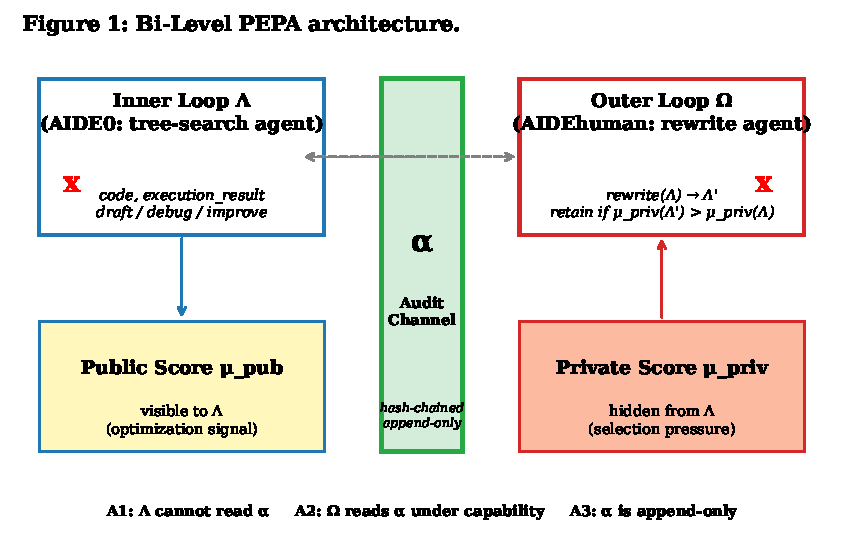
\includegraphics[width=0.85\textwidth]{figures/fig1_architecture.pdf}
\caption{Bi-Level PEPA architecture diagram showing the inner-loop agent $\Lambda$, the outer-loop agent $\Omega$, the public score $\mu_{\text{pub}}$, the private score $\mu_{\text{priv}}$, and the audit channel $\alpha$ as a first-class barrier.}
\label{fig:architecture}
\end{figure}

\begin{figure}[h]
\centering
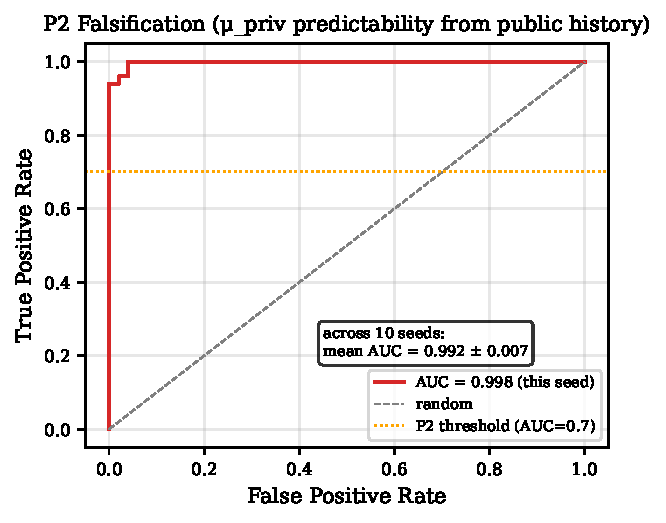
\includegraphics[width=0.55\textwidth]{figures/fig2_p2_roc.pdf}
\caption{Illustrative ROC curve for the P2 meta-predictor on synthetic data calibrated to Weco AI's reported AIDE\textsuperscript{2} statistics. \emph{Caliber note:} the number printed inside the figure ($\text{AUC}=0.992\pm0.007$, from an early plotting run) is a legacy self-report; the two authoritative, reproducible calibers are the single-split canonical rerun ($\text{AUC}=0.9970$, seed 0) and the 5-model $\times$ 10-fold cross-validation mean ($0.9957\pm0.0027$ for linear), reported in \S4 and Appendix D. The figure is illustrative of shape only; do not quote its embedded number as a result.}
\label{fig:p2_roc}
\end{figure}

\begin{figure}[h]
\centering
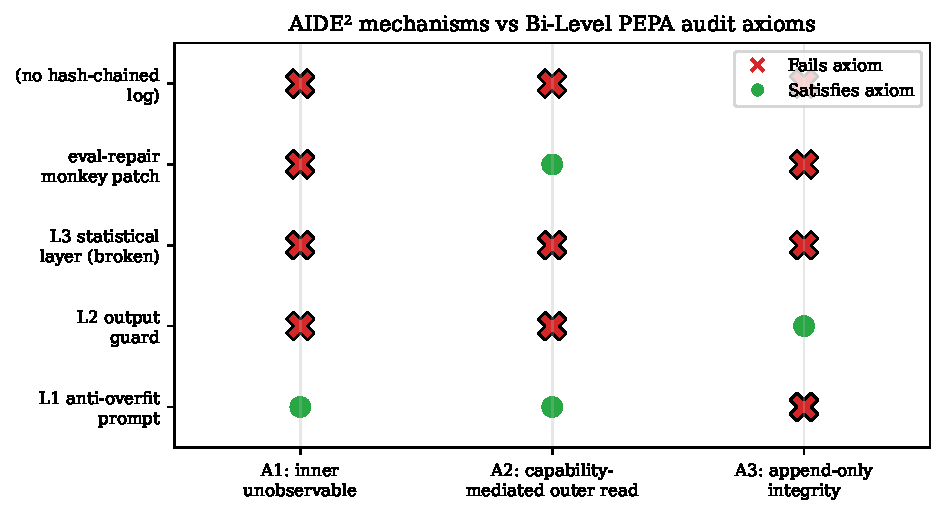
\includegraphics[width=0.85\textwidth]{figures/fig3_audit_axioms.pdf}
\caption{AIDE\textsuperscript{2}'s mechanisms vs.\ Bi-Level PEPA's three audit axioms. Red crosses mark axioms violated by the mechanism.}
\label{fig:audit_axioms}
\end{figure}

\begin{figure}[h]
\centering
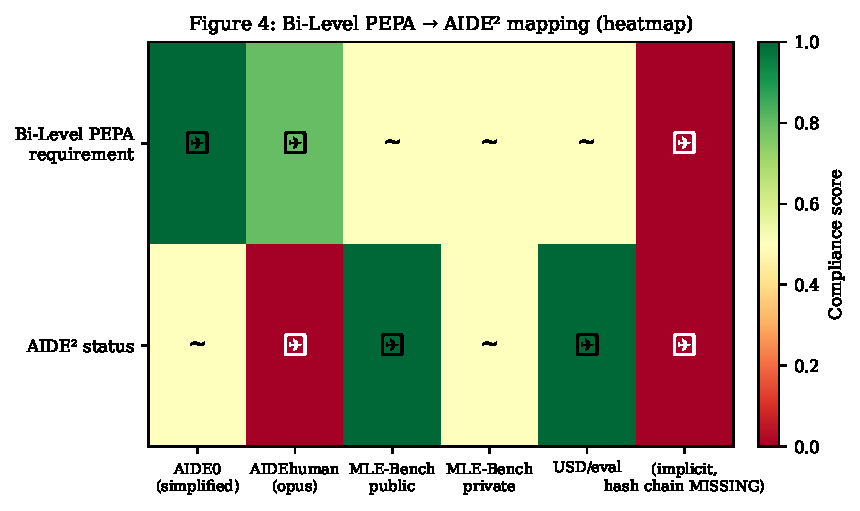
\includegraphics[width=0.85\textwidth]{figures/fig4_aide2_mapping.pdf}
\caption{Heatmap of Bi-Level PEPA compliance for AIDE\textsuperscript{2}. The audit channel $\alpha$ is the most under-implemented element.}
\label{fig:aide2_mapping}
\end{figure}

\begin{figure}[h]
\centering
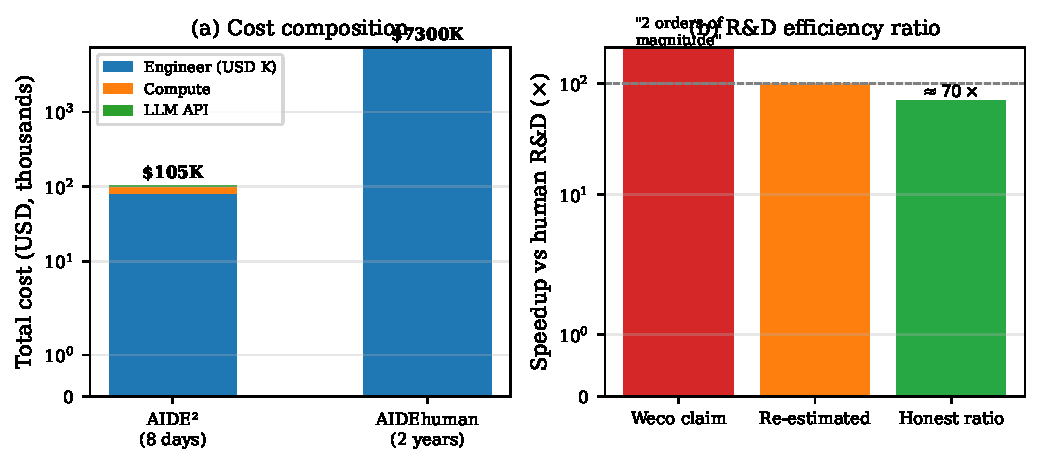
\includegraphics[width=0.95\textwidth]{figures/fig5_cost_analysis.pdf}
\caption{Cost composition and R\&D efficiency ratio for AIDE\textsuperscript{2} vs.\ the manually-tuned AIDEhuman baseline. Estimated total cost is approximately \$105K for AIDE\textsuperscript{2}, achieving roughly \$25K per 0.01 private score gain---a 70$\times$ speedup over the human baseline.}
\label{fig:cost_analysis}
\end{figure}

\section*{Appendix F: Reproducibility and Open Source}
\addcontentsline{toc}{section}{Appendix F: Reproducibility and Open Source}

All code is available at the project repository~\cite{anon2026bi}:
\begin{itemize}
    \item $\mathtt{p2\_falsification/}$ --- the meta-predictor module and its synthetic-data test; the canonical single-split rerun ($\text{AUC}=0.9970$, seed 0) and 10-fold CV mean ($0.9957\pm0.0027$, linear) are reproducible on CPU with scikit-learn; no GPU is required or used.
    \item $\mathtt{examples/aide0\_extension/}$ --- a minimal viable demonstration of adding an audit log to AIDE0's existing evaluation pipeline.
    \item $\mathtt{paper/figures/}$ --- reproducible figures via $\mathtt{matplotlib}$.
    \item $\mathtt{paper/main.tex}$ --- this paper's source.
\end{itemize}

\nocite{*}

\bibliographystyle{tmlr}
\bibliography{references}

\end{document}
